\documentclass[conference,compsoc]{IEEEtran}

\usepackage{epsfig,endnotes}
\usepackage{varwidth}
\usepackage{algorithm}
\usepackage{algpseudocode}
\usepackage{balance}
\usepackage{xcolor}
\usepackage{nicefrac}
\usepackage{amsmath}
\usepackage{braket}
\usepackage{bm}
\usepackage{mathtools}
\usepackage{multirow}
\usepackage{bigdelim}
\usepackage{mathtools}
\usepackage{amssymb}
\usepackage{indentfirst}
\usepackage{booktabs}
\usepackage{enumitem}
\usepackage{boxedminipage}
\usepackage{float}
\usepackage{graphicx}
\usepackage{caption}
\usepackage{cleveref}
\usepackage{subcaption}
\usepackage[normalem]{ulem}
\usepackage{xpatch}
%\usepackage{MnSymbol}
\usepackage{xspace}
\usepackage{listings}
\usepackage{mathpartir}

\usepackage[pdftex,bookmarks=true,pdfstartview=FitH,colorlinks,linkcolor=blue,filecolor=blue,citecolor=blue,urlcolor=blue,pagebackref=true]{hyperref}
    \urlstyle{sf}

\usepackage{stmaryrd}

\newlength{\saveparindent}
\setlength{\saveparindent}{\parindent}
\newlength{\saveparskip}
\setlength{\saveparskip}{\parskip}
 
 
\newenvironment{tiret}{%
\begin{list}{\hspace{2pt}\rule[0.5ex]{6pt}{1pt}\hfill}{\labelwidth=15pt%
\labelsep=5pt \leftmargin=20pt \topsep=3pt%
\setlength{\listparindent}{\saveparindent}%
\setlength{\parsep}{\saveparskip}%
\setlength{\itemsep}{0pt} }}{\end{list}}
 
\newenvironment{enum}{%
\begin{list}{{\rm (\arabic{ctr})}\hfill}{\usecounter{ctr}\labelwidth=17pt%
\labelsep=6pt \leftmargin=23pt \topsep=5pt%
\setlength{\listparindent}{\saveparindent}%
\setlength{\parsep}{\saveparskip}%
\setlength{\itemsep}{3pt} }}{\end{list}}
 
\newenvironment{newenum}{%
\begin{list}{{\rm \arabic{ctr}.}\hfill}{\usecounter{ctr}\labelwidth=17pt%
\labelsep=6pt \leftmargin=23pt \topsep=.5pt%
\setlength{\listparindent}{\saveparindent}%
\setlength{\parsep}{\saveparskip}%
\setlength{\itemsep}{5pt} }}{\end{list}}

\newcommand{\tool}{{\textsc{EzPC}}\xspace}
\newcommand{\minion}{{\textsc{MiniONN}}\xspace}
\newcommand{\bonsai}{{\textsc{Bonsai}}\xspace}
\newcommand{\R}{{\mathbb{R}}\xspace}
\newcommand{\mpc}{{2PC}\xspace}

\newtheorem{problem}{Problem}
\newtheorem{theorem}{Theorem}
\newtheorem{conjecture}[theorem]{Conjecture}
\newtheorem{definition}[theorem]{Definition}
\newtheorem{lemma}[theorem]{Lemma}
\newtheorem{proposition}[theorem]{Proposition}
\newtheorem{corollary}[theorem]{Corollary}
\newtheorem{claim}[theorem]{Claim}
\newtheorem{fact}[theorem]{Fact}
\newtheorem{remk}[theorem]{Remark}
\newtheorem{apdxlemma}{Lemma}


\newcommand{\namedref}[2]{\hyperref[#2]{#1~\ref*{#2}}\xspace}
\newcommand{\lemmaref}[1]{\namedref{Lemma}{lem:#1}}
\newcommand{\propref}[1]{\namedref{Proposition}{prop:#1}}
\newcommand{\theoremref}[1]{\namedref{Theorem}{theorem:#1}}
\newcommand{\claimref}[1]{\namedref{Claim}{clm:#1}}
\newcommand{\corolref}[1]{\namedref{Corollary}{corol:#1}}
\newcommand{\figureref}[1]{\namedref{Figure}{fig:#1}}
\newcommand{\tableref}[1]{\namedref{Table}{tbl:#1}}
\newcommand{\equationref}[1]{\namedref{Equation}{eq:#1}}
\newcommand{\defref}[1]{\namedref{Definition}{def:#1}}
\newcommand{\observationref}[1]{\namedref{Observation}{obs:#1}}
\newcommand{\procedureref}[1]{\namedref{Procedure}{proc:#1}}
\newcommand{\importedtheoremref}[1]{\namedref{Imported Theorem}{impthm:#1}}
\newcommand{\informaltheoremref}[1]{\namedref{Informal Theorem}{infthm:#1}}

\newcommand{\sectionref}[1]{\namedref{Section}{sec:#1}}
\newcommand{\appendixref}[1]{\namedref{Appendix}{app:#1}}
\newcommand{\propertyref}[1]{\namedref{Property}{prop:#1}}

\newcommand{\algoref}[1]{\namedref{Algorithm}{algo:#1}}



\newcommand{\TODO}[1]{{{\color{red} TODO: #1}}}
\newcommand{\divya}[1]{{{\color{blue} dg: #1}}}
\newcommand{\cmmt}[1]{{{\color{red} check: #1}}}
\newcommand{\nc}[1]{{{\color{purple} nc: #1}}}
\newcommand{\rs}[1]{{{\color{magenta} rs: #1}}}

\definecolor{mypink}{rgb}{1,0.2,0.4}
\newcommand{\aseem}[1]{{{\color{mypink} Aseem: #1}}}

\newcommand{\adv}{\mathcal{A}}
\newcommand{\env}{\mathcal{Z}}
\newcommand{\prot}{\Pi}
\newcommand{\real}{\mathsf{REAL}}
\newcommand{\ideal}{\mathsf{IDEAL}}
\newcommand{\simu}{\mathcal{S}}
\newcommand{\F}{\mathcal{F}}
\newcommand{\secparam}{\kappa}


%%circuits syntax
\newcommand{\gate}{\mathtt{g}}
\newcommand{\wire}{w}
\newcommand{\bval}{\tilde{r}}
\newcommand{\val}{\tilde{v}}
\newcommand{\crct}{\chi}

\lstset{ % 
    language=C,
    backgroundcolor=\color{white},   
    basicstyle=\footnotesize\ttfamily\bfseries,
    breakatwhitespace=false,
    breaklines=false,
    belowskip=-0.3cm,
    captionpos=b,                    
    commentstyle=\color{red},
    deletekeywords={...}, 
    escapeinside={\%*}{*)}, 
    extendedchars=true, 
    %% frame=single,
    keepspaces=true,
    keywordstyle=\color{blue},
    keywordstyle=[2]\color{blue},
    otherkeywords={*,...,uint,input1,input2,output,in},
    keywords=[2]{private},
    numbers=left,
    numbersep=5pt, 
    numberstyle=\tiny\color{gray}\bfseries, 
    rulecolor=\color{black},
    showspaces=false,
    showstringspaces=false, 
    showtabs=false, 
    stepnumber=2, 
    stringstyle=\color{mymauve},
    tabsize=2, 
    title=\lstname
}

\let\ls\lstinline



\begin{document}
\title{\tool: Programmable, Efficient, and Scalable Secure Two-Party Computation}


% author names and affiliations
% use a multiple column layout for up to three different
% affiliations
% \author{\IEEEauthorblockN{Michael Shell}
% \IEEEauthorblockA{School of Electrical and\\Computer Engineering\\
% Georgia Institute of Technology\\
% Atlanta, Georgia 30332--0250\\
% Email: http://www.michaelshell.org/contact.html}
% \and
% \IEEEauthorblockN{Homer Simpson}
% \IEEEauthorblockA{Twentieth Century Fox\\
% Springfield, USA\\
% Email: homer@thesimpsons.com}
% \and
% \IEEEauthorblockN{James Kirk\\ and Montgomery Scott}
% \IEEEauthorblockA{Starfleet Academy\\
% San Francisco, California 96678-2391\\
% Telephone: (800) 555--1212\\
% Fax: (888) 555--1212}}



\maketitle
% \begin{abstract}
% The abstract goes here.
% \end{abstract}
\IEEEpeerreviewmaketitle


\graphicspath{{./Images/}}
\DeclareGraphicsExtensions{.pdf,.jpg,.png}

\section{Introduction}
\label{sec:intro}
Today it is hard for developers to create secure implementations using cryptographic techniques.
Typical developers lack an understanding of cryptography protocols
and cannot be expected to implement them correctly without tool support.
In an ideal world, a developer declares the functionality to be implemented
in a general purpose programming language and an automatic tool takes care
of all the cryptography and generates a secure and efficient implementation  of the functionality. 
This paper provides a language-based solution to make
secure multiparty computation (SMC) accessible to the software developer community. \nc{Why do we call it SMC? A bit non-standard for crypto audiences isnt it?} \divya{I drank my tears and a part of me died when I did this. Apparently thats what it is called outside the theory community.}

%Most cryptographic tools rely on circuit as abstractions for any general computation but real-life developers write programs. It is critical to address this fundamental  representation gap to make cryptography accessible to non-crypto specialist developers. In this work, we address this gap for the case of secure multi-party computation.

%Most cryptographic tools are very hard to use non-crypto specialist developers. The task becomes even more tedious and error-prone for the case of secure multiparty computation since different protocol implementations require the function to be expressed in different representations such as Boolean or Arithmetic circuits. To make cryptography accessible to non-crypto specialist developers, we need to design systems that do crypto automatically and satisfy the properties of ... 

Secure multi-party computation \cite{yao,gmw} (SMC) is a powerful cryptographic tool that allows a set of mutually distrusting parties to compute a joint function of their secret inputs. Examples of these include various machine learning prediction algorithm where one party holds the secret input such as a medical report and the other party holds the ML model for disease prediction. Since the introduction of SMC in 1980's, there has been a large body of work \cite{..} that has transformed SMC from a mere theoretical tool to something practically efficient and usable. Hence, there have been efforts to make SMC accessible to non-specialist programmers. To understand the state-of-the-art, let us consider the following toy example.

Suppose a developer wants to compute $w^Tx >0$ securely using SMC. With the current techniques, he has two options. \nc{The two options appear quite far apart in the text. Can we make bullet points maybe?} \divya{Bullet list would look bad. I tried listing both options first and then discussing but its hard to talk about ABY before.} He can code up the functionality in a programmer friendly domain-specific language such as \cite{lambdaps,wysteria,oblivm} that would automatically compile it to an SMC protocol. The downside is that all of these works build on a cryptographic back-end that is either entirely boolean \cite{yao,gmw} or entirely arithmetic \cite{homo}. The efficiency of the generated SMC protocol is hence, bounded by the possibility of efficiently representing the function in a form that is compatible with the cryptographic back-end used. For instance, over $\ell$-bit integers, multiplication requires a boolean circuit of size  $O(\ell^2)$. 
For better efficiency, we would like to evaluate $w^Tx$ using an Arithmetic circuit and the comparison using a boolean circuit.
In fact, most interesting functions require a mix of arithmetic and boolean computations.
To address this issue, recently Demmler et al. \cite{aby} gave a cryptographic protocol for SMC where the parties can mix arithmetic and boolean computations. \footnote{Need to note somewhere that many works combined HE and Yao. Look at ABY for references.}
Hence, the second option is to write the functionality in the system developed in \cite{aby}.
However, using their system requires the programmer to be aware of complex trade-offs between arithmetic and boolean cryptographic schemes and split the functionality into such parts accordingly. In their framework, the programmer is required to write circuits consisting of  arithmetic and boolean gates along with appropriate conversion gates. In short, the current system of ABY is not suitable to be used by non-specialist programmers. 
\nc{Also say that the programmer would need to know which functionality is better suited for arithmetic/boolean and also how to split the complete functionality into such parts.}
Now the third option is to hire a cryptographer to design specialised protocols for the functionalities. 
In our work, we achieve the best of all options. \divya{add a word like automatically..}
\nc{Should we also say here that a third option is to hire a cryptographer and build specific crypto protocols for the functionalities? :) This seems to be the option we are targeting when we show our comparisons and we say that we beat or match hand-crafted protocols} \divya{We can do this! Might have to see the flow.}


%Unfortunately, implementing functionalities using SMC protocols requires thorough understanding of cryptography. To allow for widespread use of SMC, it is critical that SMC protocols are programmable by non-cryptographic experts. To cater to this, there have been several efforts developing domain-specific languages that are programmer friendly and compile to a SMC protocol. Most notable of these domain specific languages and systems include \cite{...}. All of these works build on a cryptographic back-end that is either entirely boolean \cite{yao,gmw} or arithmetic \cite{homo}. In fact, most of these works use boolean circuits based scheme for completeness\footnote{Note that comparisons cannot be expressed in arithmetic circuits}. However, most interesting functions require a mix of arithmetic and boolean computations.  Examples include ......... As one can expect, compiling these programs to boolean circuits is one of the biggest efficiency bottlenecks. \divya{Our work addresses this performance bottleneck.}

%To address this issue \divya{on the cryptographic side}, recently Demmler et al. \cite{aby} gave a cryptographic protocol for SMC where the parties can mix arithmetic and boolean computations and claimed potentially great performance benefits. However, using their system requires the programmer to be aware of trade-offs of arithmetic and boolean cryptographic schemes. In their framework, the programmer is required to write circuits consisting of a mix of arithmetic and boolean gates along with appropriate conversion gates. In short, as is also mentioned by the authors themselves, the current system is not suitable to be used by non-specialist programmers.


%%%%%%%Recent works \cite{aby,secureml,minion} have shown that great performance benefit can be obtained by mixing arithmetic and boolean computations in the back-end. Certain computations such as integer multiplication are efficient when implemented using arithmetic SMC \cite{gmw} whereas max(x,0) needs to be computed using a boolean back-end \cite{yao}. More details later.. ABY \cite{aby} requires programmer to be aware of arithmetic and boolean trade-offs and  write high-level circuits consisting of both arithmetic and boolean gates and share-conversion gates. Other works such as \cite{secureml,minion} build on ideas from \cite{aby} and develop tailor made algorithms for neural network training and prediction \cite{ml} and claim huge improvements over only boolean implementations. As is already mentioned in these works, their systems are mere proofs-of-concept and far from being implementable.

In this work, we develop and implement our framework \tool \nc{I still like EasyPC :)} \divya{I agree that \tool is bad. What would be the full form for EasyPC? Shouldn't it be EasySC?} for secure computation that achieves generality, performance and programmer productivity. The programmer writes a high level \divya{C-like} program (instead of a circuit) to describe the function to be computed. Our compiler automatically generates an SMC protocol using a mix of Arithmetic and Boolean compute. Our compiler is general and can work with any secure implementation of a mix of arithmetic and boolean computations. In our work, we focus on semi-honest secure two-party computation. We build on ABY \cite{aby} that provides the suitable cryptographic back-end in this setting. We provide a formal type system and prove correctness and security of our compiler. We evaluate our system on various benchmarks such as logistic regression and convolutional neural network (CNN) for MNIST data \cite{minionn}, naive bayes, decision trees from \cite{shafindss}. Evaluations show that protocols generated by our compiler match the performance of hand-crafted protocols in most cases (see \sectionref{sec:eval}). \divya{Below, we will  give an overview of \tool and describe our contributions in more detail.}

%The programmer is oblivious of the cryptographic back-end being used. Our compiler automatically compiles it to a circuit framework consisting to both arithmetic and boolean gates as well share-conversion gates wherever required. We use ABY as the cryptographic backend. \divya{Say something about what kind of backend we want. provides SMC for a mix of arithmetic and boolean circuit with appropriate secure conversion between two types and ABY provides such a framework for semi-honest 2pc.} Our work is compatible with malicious, multiparty as well... etc We give a type system, correctness ..... We evaluate our framework on ... and show performance comparable and even better than tailor made protocols. It is simple to program in our framework and our work provides a meaningful baseline for future works designing tailor made protocols for specific functionalities.

\subsection{\tool: Overview and Contributions} 
\label{sec:contrib}
%Write high level overview of programming language and tool.. \divya{have some preamble}
\divya{I can add paragraph headings..}

\tool is a programmer-friendly framework to express the function to be computed and uses a mix of arithmetic and boolean SMC back-ends. We illustrate the above toy example of $w^Tx >b$ in our language in \figureref{ex-sml}. As is clear from the code, the programmer is not required to write keywords such as {\em secret} or {\em public} and can remain completely oblivious of the cryptographic back-end. In contrast, \figureref{ex-aby} illustrates the same example using the framework in ABY \cite{aby}. Here, as already mentioned, the programmer needs to write the low level gates like $\mathrm{MULT, ADD, CONS, GT}$, etc. The programmer is also required to use the appropriate share conversion gates such as A2Y that converts Arithmetic shares to Yao shares. 

Our compiler is aware of cryptographic costs of different representations and inter-conversions.  Based on these costs, our compiler, given a program in \tool, automatically picks Arithmetic and Boolean representations for different sub-parts of the program and inserts the required inter-conversions as well. 
Our experiments show that automatically generated protocols using \tool match the performance of tailor-made protocols in \cite{minionn,shafindss} (see \sectionref{eval}). This shows that  \tool achieves generality, performance and programmer productivity. These features allow us to evaluate our system on a variety of benchmarks, especially, state-of-the-art ML prediction algorithms with \emph{real} data and models. 

We give a formal {\em type system} for our language and prove useful properties. We prove that if a program type checks in our language then it would run correctly, e.g., there would not be any array index out of bounds error. The programmer writes a single code describing the inputs from each party and the function to be computed. Our compiler automatically generates separate executables for the server and the client that can be executed in the distributed setting. We prove the {\em correctness} for this compilation, i.e., the outputs obtained in the distributed execution are identical to the stand-alone execution by a trusted third party. We formally reduce the {\em security} of our system to the security of the cryptographic back-end. For details on formal language, correctness and security theorems see \sectionref{ld}.
\nc{Shall we have paragraph heads or something to outline the different contributions? Above feels like one big story.}

Another issue in adoption of SMC is difficulty in scaling to large programs. 
%In general, SMC implementations struggle in scaling to large programssize of memory on a system limits the largest compute inside the SMC and hence,. 
The reason being all SMC implementations use a circuit-like representation as an intermediate representation. Hence, the largest compute that can be done securely is upper-bounded by the largest circuit that can fit in memory on a machine. \nc{Should we point out here that ABY itself has an explicit limit on circuit size and also give an example of a program that easily surpasses this bound? Also, hadnt ABY also said something about this? If so, we can mention this.}
To address this issue, we develop a technique called \emph{pipelining} that allows us to run aribitrarily large programs. At a high level, we break the original program into a sequence of small sub-programs and mask the intermediate outputs using secure secret sharing between the two parties. We appropriately append the share-reconstruction function to the beginning of the subsequent sub-program. Now, we execute each of these sub-programs sequentially in our framework. We provide details of pipelining and prove the correctness and security of this transformation in \sectionref{pipe}.

Finally, our framework \tool can serve as a meaningful baseline for future works on hand-crafted SMC protocols for specific functionalities such as \textsc{MiniONN} \cite{minionn}. 
Prior to our work, garbled circuit based two-party computation is cited as the most practical approach and used as the baseline for comparison of performance. But, it has been observed multiple times this approach does not even scale on realistic examples.



%\newpage
%\divya{ideally have small paragraphs about key features}
%1. ease to programming.. refer to section with example in our language; contrast to verilog paper; programmer is completely oblivious of security; looks like a normal/vanilla/ regular C program;
%Moreover, the developer does not write keywords such as secret and public; 
%
%
%2. first programmable system that supports a mix of arithmetic and boolean for efficiency give example of multiplication of integers; linear algebra; logistic regression and evaluate on state of the art ML prediction tasks
%
%3. prove correctness, type system guarantees correct termination, progress etc..; 
%
%%In contrast with most systems that require a programmer to label variables as public secret, we automatically infer them. leads to more efficiency compared to default secret
%
%If program type-checks then runs correctly for example no array out of bound errors
%code runs correctly in distributed env
%programmer writes one code; compiles to server code and client code
%we prove and outputs identical to stand-alone output
%distributed code produces same output as if the code were run by distributed third party
%
%
%4. Scaling to large programs. Describe pipeling here... Like all MPC implementations use an intermediate rep as a circuit and largest compute that can run is given by largest circuit that can fit in memory are restricted by memory of machines. This in turn limits the size of functions 
%We implement/give/design a generic technique called pipelining that allow us to run arbitrarily large computations without affecting security.
%
%
%5. Previous papers when comparing with generic 2pc compare with Yao; does not scale etc...
%can serve as a baseline for future works on hand-crafted algorithms for specific applications cite minion etc here...
%




\vspace{10pt}

\noindent\textbf{Related Work} \divya{I think we should say a few words here about the following: minionn, verilog paper, 
\cite{lambdaps,wysteria}

}


\newpage
\begin{figure}
\begin{verbatim}
uint w[30];
uint b;
uint x;
for i = [0:30] {
        w[i] = input1();
}
b = input1();
for i = [0:30] {
    x[i] = input2();
}
uint acc = 0;

for i = [0:30] {
  acc =  acc + (w[i] * x[i]);
}
output((acc > b) ? 1 : 0);
\end{verbatim}
\caption{Code in \tool for $w^Tx >b$}
\label{fig:ex-sml}
\end{figure}


\begin{figure}
\begin{verbatim}
for (uint32_t i = 0; i < 30; i++)
{
    share * s_a_tmp_0 = acirc->
    					PutMULGate( s_a_a[i] , s_a_b[i] );
    s_a_j = acirc->
    		PutADDGate( s_a_j , s_a_tmp_0 );
}

share *s_y_j = ycirc->PutA2YGate( s_a_j );
uint32_t _tmp_2 = 1<<31-1 ;
share * s_y__tmp_2 = ycirc->PutCONSGate
					( _tmp_2 ,bitlen);
share * s_y_tmp_1 = ycirc->PutGTGate
					( s_y_j , s_y__tmp_2 );
uint32_t _tmp_3 = 1 ;
share * s_y__tmp_3 = ycirc->PutCONSGate
					( _tmp_3 ,bitlen);
uint32_t _tmp_4 = 0 ;
share * s_y__tmp_4 = ycirc->PutCONSGate
					( _tmp_4 ,bitlen);
share * s_y_k = ycirc->PutMUXGate
					( s_y__tmp_3 , s_y__tmp_4 , s_y_tmp_1 );
share * s_y_tmp_5 = ycirc->PutOUTGate
					( s_y_k , ALL);
party->ExecCircuit();
uint32_t _output = s_y_tmp_5->
			get_clear_value<uint32_t>();
\end{verbatim}
\caption{Code in ABY}
\label{fig:ex-aby}
\end{figure}

\section{\tool Overview}
\label{sec:ex}
%$w^Tx>0$, mnist logistic regression
%% \divya{add reference to before and later... as mentioned we would run evaluations on secure prediction of different models. Here we describe scenario in detail..}

\begin{figure}
  %\vspace{-20pt}
  %\begin{center}
  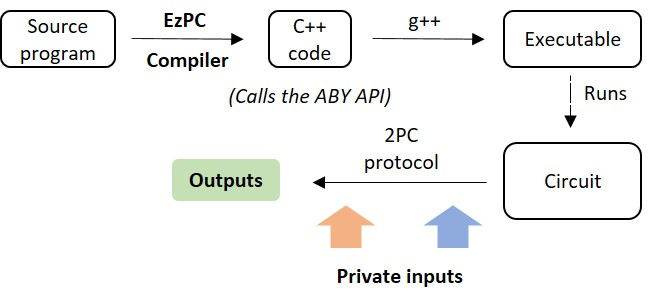
\includegraphics[width=0.45\textwidth]{toolchain}
  %\end{center}
  %\vspace{-20pt}
\caption{\tool toolchain}
\label{fig:toolchain}
\end{figure}

Figure~\ref{fig:toolchain} shows an overview of the \tool
toolchain. We give a brief overview of each of these phases below.

\subsubsection*{Source language}
Consider the example $w^Tx >b$ from Section~\ref{sec:intro}, where
$w$ and $b$ constitute the server's input (a classifier) and $x$ is
the client's input vector. Figure~\ref{fig:ex-sml} shows \tool code
for this example. The code first reads the inputs of the two parties
using the \ls{input1} and \ls{input2} expressions. It then uses a
\ls{for} loop to compute \ls{acc}, the dot product of \ls{w} and
\ls{x}. Finally, the code outputs the result of comparing \ls{acc}
with \ls{b} only to the client.

\tool source language is a simple, imperative language that enables
the programmers to express \mpc computations in terms of their
``ideal'' functionalities, without dealing with any cryptographic
details. The languages provides multi-dimensional arrays, conditional
expressions (the ternary $?\::$ operator), \ls{for}~loops,
\ls{if}~statements, and special syntax for input/output.

\begin{figure}
\begin{verbatim}
for (uint32_t i = 0; i < 30; i++)
{
    share * s_a_tmp_0 = acirc->
    					PutMULGate( s_a_a[i] , s_a_b[i] );
    s_a_j = acirc->
    		PutADDGate( s_a_j , s_a_tmp_0 );
}

share *s_y_j = ycirc->PutA2YGate( s_a_j );
uint32_t _tmp_2 = 1<<31-1 ;
share * s_y__tmp_2 = ycirc->PutCONSGate
					( _tmp_2 ,bitlen);
share * s_y_tmp_1 = ycirc->PutGTGate
					( s_y_j , s_y__tmp_2 );
uint32_t _tmp_3 = 1 ;
share * s_y__tmp_3 = ycirc->PutCONSGate
					( _tmp_3 ,bitlen);
uint32_t _tmp_4 = 0 ;
share * s_y__tmp_4 = ycirc->PutCONSGate
					( _tmp_4 ,bitlen);
share * s_y_k = ycirc->PutMUXGate
					( s_y__tmp_3 , s_y__tmp_4 , s_y_tmp_1 );
share * s_y_tmp_5 = ycirc->PutOUTGate
					( s_y_k , ALL);
party->ExecCircuit();
uint32_t _output = s_y_tmp_5->
			get_clear_value<uint32_t>();
\end{verbatim}
\caption{Code in ABY}
\label{fig:ex-aby}
\end{figure}

\subsubsection*{\tool compiler}
\tool compiler takes as input a source program and produces a C++
program as output. Figure~\ref{fig:ex-aby} shows the output code for
the example in Figure~\ref{fig:ex-sml}. The output program
contains party-specific code for inputs and outputs
(\ls{role == SERVER} and \ls{role == CLIENT}), and common code for the
computation.

The compiler splits the input
program into \emph{public} and \emph{secret} components. The public
components translate into regular C++ code, while the secret
components translate into API calls into our crypto back-end
(ABY). For instance, for the code in Figure~\ref{fig:ex-sml}, the \tool
compiler realizes that the array index \ls{i} in the dot product loop
is public, and hence the array accesses need not be compiled
obliviously. Therefore, it compiles the \ls{for}~loop into a C++
\ls{for}~loop that will be executed in-clear
(line~\ref{line:dotproductloop}).

Within the secret components, the \tool compiler is ``cryptographic
cost-aware'', and appropriately picks either arithmetic or boolean
circuit representations for different sub-componenets. For example,
the compiler realizes that the dot product computation is more
efficient in the arithmetic representation, and therefore it builds
the corresponding circuit using the arithmetic circuit builder
\ls{acirc} (lines~\ref{line:dotmulgate} and~\ref{line:dotaddgate}). On
the other hand, since the comparison with \ls{b}, and the conditional
expression computation are more efficient in the boolean
representation, the \tool compiler uses the Yao circuit builder
\ls{ycirc} to build the corresponding circuits
(lines~\ref{line:condyaobegin} to~\ref{line:condyaoend})\footnote{As
  we mention in
  Section~\ref{sec:impl}, in our usage of ABY, boolean is synonymous
  with Yao.}.

Importantly, conversions between the arithmetic and boolean
represenation require share-conversions. The \tool compiler also
instruments these conversion gates accordingly. For example, in
lines~\ref{line:convacc} and~\ref{line:convb}, the compiler converts
\ls{a_acc} and \ls{a_b} to boolean representation, before they are
input to the comparison and multiplexer circuits.

\subsubsection*{Circuit generation and evaluation} The next step in
\tool is to
compile the output C++ code and execute it. Doing so reduces away the
public parts of the program, including the array accesses, and
generates a \mpc circuit comprising of arithmetic and boolean gates,
with appropriate conversion gates. The circuit is then evaluated using
a \mpc protocol.

We can now concretely see the advantages of \tool. Unarguably, it is
easier for a developer to program, and get right, the code in
Figure~\ref{fig:ex-sml}, rather than the code in
Figure~\ref{fig:ex-aby} (as we mentioned in Section~\ref{sec:intro},
other high-level languages are limited in their use of a single,
arithmetic or boolean, crypto back-end). \tool also enables the
programmer to easily modify their code, while the compiler takes care
of efficiency. For example, consider in Figure~\ref{fig:ex-sml} a
change from multiplication to bitwise OR in the \ls{for} loop. It
turns out that once that's the case, it is more efficient to do both
the addition and bitwise OR using boolean circuits (if the addition is
still done using arithmetic, the conversion cost starts to take
over). In \tool, the programmer simply needs to change one operator in
the source code, and the compiler generates efficient code that uses
boolean addition. Whereas, if the programmer was writing ABY
code, she either has to sacrifice performance, or she would have to
revisit many parts of the circuit and change them.

To summarize, \tool raises the level of abstraction for the
programmers, and generates efficient crypto protocols automatically,
while its metatheory provides strong correctness and security
guarantees.

%% Consider a  cloud service provider Bob that wants to provide a service to diagnose
%% whether a patient has breast cancer or not. Bob trains a machine learning classification model
%% that results in a vector $w$ (say of length 30) and a scalar $b$.
%% This model is the intellectual property of Bob and he  wants to keep it secret.
%% Given a patient's medical report, in the form of a vector $x$ (also of length 30),
%% the classifer predicts that the patient has breast cancer if $w^Tx>b$.
%% However, for this task Bob needs access to $x$, which is private data of a customer.

%% A potential customer Alice might not want to reveal $x$ to Bob because of privacy concerns.
%% And Bob does not want to reveal $w$ and $b$ because then Alice can steal the model. \divya{Use HIPAA compliance; as it can leak information of patients that was used in training; more compelling argument. See Shafi intro.}
%% SMC can help Alice and Bob compute $w^Tx>b$ securely, such that Alice receives the classifier's
%% prediction and Bob learns nothing about $x$. Moreover, Alice does not learn anything more about $w$
%% and $b$ than what is revealed by the prediction. 
%% \nc{This is a bit repetitive from the intro, isnt it? Should we have another example perhaps?}
%% To implement this system, Bob can write the code in \tool and this code is shown in Figure~\ref{fig:ex-sml}.
%% The expression {\tt input1} reads a value from Bob and {\tt input2} reads from Alice.
%% The language has arrays and simple loops. A loop {\tt for i = [0:N]} repeats its
%% body {\tt N} times, the loop counter {\tt i} is assigned {\tt 0} in the first iteration,
%% and is incremented by one after each iteration. Unbounded {\tt while} loops are problematic
%% from a cryptographic standpoint and our language only permits these simple {\tt for} loops. 
%% The first loop in Figure~\ref{fig:ex-sml} reads the model $w$ from Bob, the second loop reads
%% Alice's medical report $x$, and the third loop computes the dot product $w^Tx$.
%% The last {\tt output} statement sends the result of the comparison $w^Tx>b$ to Alice.
%% In particular, the ternary ``{\tt ? :}" operator performs a branch and the result is the second (third)
%% argument if the first argument is true (false).

%% The \tool compiler is fully automatic and compiles the code described in Figure~\ref{fig:ex-sml} to the C++ code that makes calls to the ABY library  in
%% Figure~\ref{fig:ex-aby}. An alternative to using \tool is to directly write this C++ code.
%% However, this code is much more complex than the implementation written in \tool.
%% Therefore, it is difficult for Alice and bob to verify its correctness and security.
%% Unlike \tool implementations, the ``secret" variables containing private data ({\tt w,x,b,acc}) need to be handled differently compared to ``public" variables such as loop counters ({\tt i}). In particular, the former are manipulated by the ABY library and the latter are manipulated like standard  C++ variables.
%% Additionally, the C++ code branches on  the special variable
%% {\tt role}  to decide whether the enclosing code is executed by the {\tt SERVER} Bob or by
%% the {\tt CLIENT} Alice. In Figure~\ref{fig:ex-sml}, the developer does not need to
%% manipulate {\tt role} explicitly. In addition to simplifying the implementation, \tool prevents developers from writing buggy code such as\\
%% \verb+if(role == SERVER) {...manipulate x...}+

%% Furthermore, the code in Figure~\ref{fig:ex-aby} is too low level.
%% In particular, it is first builds a circuit that represents the computation
%% $w^Tx>b$ and then executes it via a call to {\tt ExecCircuit}.
%% To build a circuit, the code adds multiplication gates ({\tt PutMULGate})
%% and addition gates ({\tt PutADDGate}) for the dot product.
%% Subsequently, it uses a ``greater than" gate ({\tt PutGTGate})
%% and a multiplexer gate ({\tt PutMUXGate}) for the comparison with $b$.
%% For efficiency, the operations for dot product need to be performed using 
%% arithmetic circuits. However, ABY's arithmetic circuits cannot express
%% comparisons and these need  boolean circuits.
%% A program that uses both arithmetic circuit and boolean circuits
%% requires conversion gates that help  interconvert between arithmetic
%% representations and boolean representations ({\tt PutA2YGate}).
%% Bigger computations often require multiple conversions and the
%% developer effort can quickly become significant.

%% Moreover, it is difficult to maintain the code in Figure~\ref{fig:ex-aby}.
%% For example, if the multiplication is changed to a bitwise-or then,
%% in the absence of \tool, an efficiency-conscious developer would need to  use boolean circuits everywhere and would be tasked with removing all arithmetic circuits and the interconversion gates (the cost of  conversion overweighs the gains of performing an arithmetic addition instead of a boolean addition). 
%%  With \tool, the developer needs to change only a single character (replace {\tt *} in Figure~\ref{fig:ex-sml} with {\tt |}) to achieve the same effect. 
%% On this example and other small examples, we have found that the compiler generated C++ code from a \tool implementation is as efficient as manually written C++ code. In particular, for $w^Tx>b$, the compiler automatically generates code that uses arithmetic circuits for dot product and inserts appropriate conversion gates. Finally, although this paper uses ABY for evaluation, the  compiler can be easily retargeted to generate code for other cryptography backends.


%% The \tool compiler provides strong static guarantees. For example, a well typed
%% \tool program is guaranteed to execute to termination without errors. A \tool program cannot go into non-termination or dereference illegal memory, i.e., no buffer overflows or underflows can happen at run time. Production compilers such as {\tt gcc} provide no such guarantees
%% for the code in Figure~\ref{fig:ex-aby}.
%% The primary reason that we are able to achieve these guarantees is because
%% \tool has been designed to be verifiable and is backed by formal semantics. 
%% Furthermore, the compiler output is guaranteed to be a cryptographically secure
%% implementation of the functionality declared by the \tool code. 
%% Moreover, the \tool compiler also generates a C implementation that can be run natively on a single machine for functional testing. 


%\newcommand{\kw}[1]{{\lstinline[basicstyle=\small\color{blue}]{#1}}}
\newcommand{\kw}[1]{{\ensuremath{\mathtt{#1}}}}
\newcommand{\ftext}[1]{\text{\small{#1}}}
\newcommand{\cond}[3]{\ensuremath{{{#1}\:?\:{#2}\::{#3}}}}
\newcommand{\for}[4]{\ensuremath{\kw{for}\:{#1}\:\kw{in}\:[{#2}, {#3}]\:\kw{do}\:{#4}}}
\newcommand{\ite}[3]{\ensuremath{\kw{if}({#1}, {#2}, {#3})}}
\newcommand{\loops}[3]{\ensuremath{\kw{while}\:{#1} \leq {#2}\:\kw{do}\:{#3}}}

\section{Formal development}
\label{sec:ld}



%In this section we prove the correctness and security of our compiler.
%%
%We first formalize the source and target languages. Our source runtime
%semantics is a model of the ideal, trusted third-party semantics, and
%generates observations corresponding to the values revealed to the
%parties.
%%
%The target language semantics (a model of the C++ code generated by
%our compiler implementation) ``computes away'' the public parts and
%arrays from the compiled program, generating a secure computation
%circuit. Crucially, this semantics does not have access to the secret
%inputs--those are processed by the secure computation circuit.
%%
%Finally, we formalize the circuit semantics that computes the
%generated circuit, and like the source semantics, emits observations
%corresponding to the values revealed to the parties.
%
%We then present the compilation rules. To prove the correctness
%of our compiler, we prove that it preserves the observations. For
%security of our compiler, we reduce the security argument to the
%security of the cryptographic protocol used to compute the secure
%computation circuit.
%\nc{Should we also say that security relies on correctness? (they go together)}
%We present only selected parts of our formalization for space
%reasons. Full definitions and proofs can be found in the supplementary
%material submitted along with the paper.


In this section we prove correctness and security of our \tool compiler.
We formalize our source, intermediate and circuit languages. 
An example of a program in our source language is provided in \figureref{ex-sml}.
%Our source runtime semantics is a model of the ideal, trusted third-party semantics, and
%generates observations corresponding to the values revealed to the
%parties.
Our source runtime semantics describe the ``trusted third party" execution semantics of the source programs and
generate observations corresponding to the values revealed to the
parties.
%
We present the compilation rules that type check a program in the source language and generate a program in the intermediate language. This intermediate language models programs such as \figureref{ex-aby} generated by our compiler implementation.
%
We evaluate the program in our intermediate language  to a circuit by ``evaluating away'' the public parts and the arrays. Crucially, this step does not have access to the secret inputs; those are processed by the distributed circuit semantics that model the \mpc back-end.
%
Evaluation in the distributed setting involves the parties running an interactive protocol. This step, like  the source semantics, emits observations corresponding to the values revealed to the parties. 
%Finally, we formalize the distributed circuit semantics (of the cryptographic back-end) that computes the generated circuit in the distributed setting, and like  the source semantics, emits observationscorresponding to the values revealed to the parties.

To prove the correctness of \tool, we prove that  the observations in source semantics and distributed circuit semantics are identical (see \theoremref{correctness}). 
We combine this correctness guarantee and the security of the \mpc back-end to argue security of the implementations generated by \tool (see \theoremref{security}).
%For the security of our compiler, we rely on the correctness guarantee and  reduce the security to the security of the underlying cryptographic protocol used to compute the generated circuit (see \theoremref{security}).
We present only selected parts of our formalization for space
reasons. Full definitions and proofs can be found in~\cite{anonymized}.


%\TODO{Do we want to write things in logical order or order in paper?}



\begin{figure}
  \small
  \[
  \begin{array}{rrcl}
    \ftext{Base type} & \sigma &::=& \kw{uint} \mid \kw{bool}\\
    \ftext{Type} & \psi &::=& \sigma \mid \sigma[n]\\
    \ftext{Constant} & c &::=& n \mid \top \mid \bot\\
    \ftext{Expression} & e &::=& c \mid x \mid e_{1} \mulop e_{2} \mid e_{1} > e_{2} \mid \cond{e_{1}}{e_{2}}{e_{3}}\\
    & &\mid& [\overline{e_{i}}]_{n} \mid x[e] \mid \kw{in}_{j}\\
    \ftext{Statement} & s &::=& \psi\:x = e \mid x := e \mid \for{x}{n_{1}}{n_{2}}{s}\\
    & & \mid& x[e_{1}] := e_{2} \mid \ite{e}{s_{1}}{s_{2}} \mid \kw{out}\:e \mid s_{1}; s_{2}\\
    & & \mid& \loops{x}{n}{s}
  \end{array}
  \]
\caption{Source language syntax}
\label{fig:srclang}
\end{figure}

\begin{figure}
  \small
  \fbox{$\rho \vdash e \Downarrow v$}
  \[
  \\
  \begin{array}{c}
    \inferrule*[lab={\footnotesize{E-Var}}]
               {
               }
               {
                 \rho \vdash x \Downarrow \rho(x)
               }
               
               \hspace{0.1cm}
               
    \inferrule*[lab={\footnotesize{E-Mult}}]
               {
                 \forall i \in \{1, 2\}.\:\rho \vdash e_{i} \Downarrow n_{i}
               }
               {
                 \rho \vdash e_{1} \mulop e_{2} \Downarrow n_{1} \mulop n_{2}
               }

               \hspace{0.1cm}
               \inferrule*[lab={\footnotesize{E-Cond}}]
               {
                 \rho \vdash e \Downarrow c\\\\
                 c = \top \Rightarrow e' = e_{1}\\\\
                 c = \bot \Rightarrow e' = e_{2}\\\\
                 \rho \vdash e' \Downarrow c'
               }
               {
                 \rho \vdash \cond{e}{e_{1}}{e_{2}} \Downarrow c'
               }
               
   
\\\\
	 \inferrule*[lab={\footnotesize{E-Read}}]
               {
                 \rho \vdash x \Downarrow [\overline{c_{i}}]_{n_{1}} \\\\
                 \rho \vdash e \Downarrow n \quad n < n_{1}
               }
               {
                 \rho \vdash x[e] \Downarrow c_{n}
               }
    
               \hspace{0.1cm}
    \inferrule*[lab={\footnotesize{E-Arr}}]
               {
                 \forall i \in [n].\:\rho \vdash e_{i} \Downarrow c_{i}
               }
               {
                 \rho \vdash [\overline{e_{i}}]_{n} \Downarrow [\overline{c_{i}}]_{n}
               }
               \hspace{0.1cm}
    \inferrule*[lab={\footnotesize{E-Inp}}]
               {
               }
               {
                 \rho \vdash \kw{in}_{j} \Downarrow c
               }
  \end{array}
  \]
  \\\\
    \fbox{$\rho \vdash s \Downarrow \rho'; O$}
  \[
  \\
  \begin{array}{c}
    \inferrule*[lab={\footnotesize{E-Decl}}]
               {
                 \rho \vdash e \Downarrow v
               }
               {
                 \rho \vdash \psi\:x = e \Downarrow \rho, x \mapsto v; \cdot
               }
               
               \hspace{0.1cm}

    \inferrule*[lab={\footnotesize{E-LoopT}}]
               {
                 \rho(x) > n
               }
               {
                 \rho \vdash \loops{x}{n}{s} \Downarrow \rho; \cdot
               }

               \\\\
               
    \inferrule*[lab={\footnotesize{E-LoopI}}]
               {
                 \rho(x) \leq n\\\\
                 \rho \vdash s \Downarrow \rho_{1}; O_{1}\\\\
                 \rho_{2} = [\rho_{1}]_{\mathsf{dom}(\rho)}[x \mapsto \rho_{1}(x) + 1]\\\\
                 \rho_{2} \vdash \loops{x}{n}{s} \Downarrow \rho_{3}; O_{2}
               }
               {
                 \rho \vdash \loops{x}{n}{s} \Downarrow \rho_{3}; O_{1}, O_{2}
               }

               \hspace{0.2cm}

    \inferrule*[lab={\footnotesize{E-If}}]
               {
                 \rho \vdash e \Downarrow c\\\\
                 c = \top \Rightarrow s = s_{1}\\\\
                 c = \bot \Rightarrow s = s_{2}\\\\
                 \rho \vdash s \Downarrow \rho_{1}; O
               }
               {
                 \rho \vdash \ite{e}{s_{1}}{s_{2}} \Downarrow \rho_{1}; O
               }

               \\\\
               
    \inferrule*[lab={\footnotesize{E-For}}]
               {
                 \rho, x \mapsto n_{1} \vdash \loops{x}{n_{2}}{s} \Downarrow \rho_{1}; O
               }
               {
                 \rho \vdash \for{x}{n_{1}}{n_{2}}{s} \Downarrow \rho_{1} - \{x\}; O
               }


               \hspace{0.2cm}

    \inferrule*[lab={\footnotesize{E-Out}}]
               {
                 \rho \vdash e \Downarrow c
               }
               {
                 \rho \vdash \kw{out}\:e \Downarrow \rho; c
               }

\end{array}
  \]
\caption{Source semantics (selected rules)}
\label{fig:srcsem}
\end{figure}

\subsubsection*{Source language} Our source language
 is a simple imperative language and we show a subset of the supported operators in \figureref{srclang}. Types
$\psi$ consist of the base types $\sigma$, and arrays
of base types $\sigma[n]$, where $n$ is the array length. Though we
model only one dimensional arrays, our implementation supports
 multi-dimensional arrays as well. Expressions $e$ in the language include the
 integer constants $n$, \kw{bool} constants $\top$ and $\bot$,
variables $x$, binary operations $e_{1} \mulop e_{2}$ and $e_{1} > e_{2}$,
conditionals $\cond{e}{e_{1}}{e_{2}}$, array literals 
$[\overline{e_{i}}]_{n}$\footnote{We write $\overline{e}$ (and
  similarly for other symbols) to denote a sequence of expressions.
The length of the sequence is usually clear from the context.}, and
array reads $x[e]$. The expression $\kw{in}_{j}$ denotes input from
party $j$. The statements $s$ in the language comprise of variable
declarations and assignments ($\psi\:x = e$ and $x := e$ resp.),
\kw{for} loops, array writes ($x[e_{1}] := e_{2}$), \kw{if}
statements, and sequence of statements ($s_{1}; s_{2}$). The statement
$\kw{out}\:e$ denotes revealing the value of $e$ to the
parties. The \kw{while} statement is an internal syntax that is not
exposed to the programmer. \\

\noindent\textbf{Source semantics.} The runtime semantics for the source language is shown in
\figureref{srcsem}. These semantics show how a ``trusted third party" computes the outputs when given the inputs of both the parties. 
 Values $v$, runtime environments $\rho$, and
observations $O$ are defined as follows:

\vspace{0.2cm}
$
\small
\begin{array}{rrcl}
    \ftext{Value} & v &::=& c \mid [\overline{c_{i}}]_{n}\\
    \ftext{Runtime environment} & \rho &::=& \cdot \mid \rho,x \mapsto v\\
    \ftext{Observation} & O & ::= & \cdot \mid c, O \\
\end{array}
$

\vspace{0.2cm}
Values consist of constants and array of constants, runtime environment
$\rho$ maps variables to values, and observations are sequences of
constants.

The judgment $\rho \vdash e \Downarrow v$ denotes the big-step
evaluation of an expression~$e$ to a value~$v$ under the runtime
environment~$\rho$. Rule ({\sc{E-Var}}) looks up the value of $x$ in
the environment. Rule ({\sc{E-Mult}}) inductively evaluates $e_{1}$ and
$e_{2}$, and evaluates to their product. Rule ({\sc{E-Read}})
evaluates an array read operation. It first evaluates $x$ to an array
value $[\overline{c_{i}}]_{n_{1}}$, and $e$ to a \kw{uint} value
$n$. It then returns $c_{n}$, the $n$-th index value in the array,
provided $n < n_{1}$, the length of the array. Rule ({\sc{E-Inp}})
evaluates to some constant $c$ denoting party $j$'s input. 
%We model the inputs to be base constants, a
An array input can be written in the
language as $[\kw{in}_{j}]_{n}$, which can then evaluate using the
rule ({\sc{E-Arr}}). The remaining rules are straightforward, and are
elided for space reasons.

The judgment $\rho \vdash s \Downarrow \rho_{1}; O$ represents the
big-step evaluation of a statement $s$ under environment $\rho$
producing a new environment $\rho_{1}$ and observations $O$. Rule
({\sc{E-Decl}}) evaluates the expression $e$ to $v$, and returns the
updated environment $\rho,x \mapsto v$, with empty observations. Rule
({\sc{E-If}}) evaluates the guard expression, and then evaluates
either $s_{1}$ or $s_{2}$ accordingly. The $\kw{for}$ statements evaluate
through the internal $\kw{while}$ syntax. Specifically, the rule
({\sc{E-For}}) appends $\rho$ with $x\mapsto n_{1}$,
evaluates $\loops{x}{n_{2}}{s}$ to $\rho_{1}; O$, and returns
$\rho_{1} - \{x\}$ (removing $x$ from $\rho_{1}$) and $O$. Rule
({\sc{E-LoopI}}) shows the inductive case for \kw{while}
statements, when $\rho(x) \leq n$. The rule evaluates $s$, producing
$\rho_{1}; O_{1}$. It then restricts $\rho_{1}$ to the domain of
$\rho$ ($[\rho_{1}]_{\mathsf{dom}(\rho)}$) to remove the variables
added by $s$, increments the value of $x$, and evaluates the
\kw{while} statement under this updated environment. Rule
({\sc{E-LoopT}}) is the termination case for \kw{while} statements,
when $\rho(x) > n$. Finally, the rule ({\sc{E-Out}}) evaluates the
expression, and adds its value to the observations.

\newcommand{\lcond}[4]{\ensuremath{{{#2}\:?_{{#1}}\:{#3}\::{#4}}}}
%\newcommand{\for}[4]{\ensuremath{\kw{for}\:{#1}\:\kw{in}\:[{#2}, {#3}]\:\kw{do}\:{#4}}}
%\newcommand{\ite}[3]{\ensuremath{\kw{if}({#1}, {#2}, {#3})}}
%\newcommand{\loops}[3]{\ensuremath{\kw{while}\:{#1} \leq {#2}\:\kw{do}\:{#3}}}

\begin{figure}
  \small
  \[
  \begin{array}{rrcl}
    \ftext{Secret label} & m &::=& \mathcal{A} \mid \mathcal{B}\\
    \ftext{Label} & \ell &::=& \mathcal{P} \mid m\\
    \ftext{Type} & \tau &::=& \sigma^{\ell} \mid \sigma^{\ell}[n]\\
    \ftext{Expression} & \widetilde{e} &::=& c \mid x \mid \widetilde{e_{1}} \mulop_{\ell} \widetilde{e_{2}} \mid \widetilde{e_{1}} >_{\ell} \widetilde{e_{2}} \\
    & & \mid & \lcond{\ell}{{\widetilde{e}}}{{\widetilde{e_{1}}}}{{\widetilde{e_{2}}}} \mid x[\widetilde{e}] \mid [\overline{\widetilde{e_{i}}}]_{n} \mid \kw{in}^{m}_{j} \mid \widetilde{e} \rhd m\\
    \ftext{Statement} & \widetilde{s} &::=& \tau\:x = \widetilde{e} \mid x := \widetilde{e} \mid \dots \mid \widetilde{s_{1}}; \widetilde{s_{2}} \mid \dots\\
  \end{array}
  \]
\caption{Intermediate language syntax}
\label{fig:interlang}
\end{figure}









\subsubsection*{Intermediate language} \figureref{interlang} shows the
intermediate language of our compiler. The syntax follows that of the source
language, except that the types and operators are \emph{labeled}. 
%Below we mainly focus on the bits that are different from the source
%language.
A label $\ell$ can be the  public label $\mathcal{P}$ or  one of the secret labels $\mathcal{A}$ or
$\mathcal{B}$, which denote arithmetic and boolean respectively.
Types $\tau$ are then
labeled base types $\sigma^{\ell}$ and arrays of labeled base types
$\sigma^{\ell}[n]$.

Most of the expression forms $\widetilde{e}$ are same as $e$, except
that the binary operators, and the conditional forms
are annotated with labels $\ell$, denoting how the operators should be
evaluated ($\mathcal{P}$ for in-clear, $\mathcal{A}$ for arithmetic circuits, and
$\mathcal{B}$ for boolean circuits). The
form $\widetilde{e} \rhd m$ denotes coercing the value of $\widetilde{e}$ to be
$m$-secret shared, which is useful for share-conversions between boolean and arithmetic and also for sharing public values. 
%The statements $\widetilde{s}$ are analogous to $s$.



\begin{figure}[t]
  \small
  \fbox{$\Gamma \vdash e : \tau \leadsto \widetilde{e}$}
  \[
  \begin{array}{c}
     \inferrule*[lab={\footnotesize{T-Cons}}]
               {
                 \tau = \mathsf{typeof}(c)^{\mathcal{P}}
               }
               {
                 \Gamma \vdash c : \tau \leadsto c 
               }
               
                \inferrule*[lab={\footnotesize{T-Inp}}]
               {
               }
               {
                 \Gamma \vdash \kw{in}_{j} : \sigma^{m} \leadsto \kw{in}^{m}_{j}
               }

   

    %% \inferrule*[lab={\footnotesize{T-Cons}}]
    %%            {
    %%              \tau = \mathsf{typeof}(c)^{\mathcal{P}}
    %%            }
    %%            {
    %%              \Gamma \vdash c : \tau \leadsto c
    %%            }

    %%  \inferrule*[lab={\footnotesize{T-Var}}]
    %%            {
    %%            }
    %%            {
    %%              \Gamma \vdash x : \Gamma(x) \leadsto x
    %%            }
\\\\

	  \inferrule*[lab={\footnotesize{T-Mult}}]
               {
                 \forall i \in \{1,2\}.\:\Gamma \vdash e_{i} : \kw{uint}^{\ell} \leadsto \widetilde{e_{i}}\\\\
                 \left(\ell = \mathcal{P}\right) \vee \left(\ell = \mathcal{A}\right)
               }
               {
                 \Gamma \vdash e_{1} \mulop e_{2} : \kw{uint}^{\ell} \leadsto \widetilde{e_{1}} \mulop_{\ell} \widetilde{e_{2}}
               }
               
     \inferrule*[lab={\footnotesize{T-Gt}}]
               {
                 \forall i \in \{1,2\}.\:\Gamma \vdash e_{i} : \kw{uint}^{\ell} \leadsto \widetilde{e_{i}}\\\\
                 \left(\ell = \mathcal{P}\right) \vee \left(\ell = \mathcal{B}\right)
               }
               {
                 \Gamma \vdash e_{1} > e_{2} : \kw{bool}^{\ell} \leadsto \widetilde{e_{1}} >_{\ell} \widetilde{e_{2}}
               }

     
\\\\               

	\inferrule*[lab={\footnotesize{T-Read}}]
               {
                 \Gamma \vdash x : \sigma^{\ell}[n] \leadsto x\\\\
                 \Gamma \vdash e : \kw{uint}^{\mathcal{P}} \leadsto \widetilde{e}\\\\
                  \models e < n
               }
               {
                 \Gamma \vdash x[e] : \sigma^{\ell} \leadsto x[\widetilde{e}]
               }


     \inferrule*[lab={\footnotesize{T-Cond}}]
               {
                 \Gamma \vdash e : \kw{bool}^{\ell} \leadsto \widetilde{e}\\\\
                 \forall i \in \{1,2\}.\:\Gamma \vdash e_{i} : \sigma^{\ell'} \leadsto \widetilde{e_{i}}\\\\
                 \ell = \mathcal{P} \vee (\ell = \mathcal{B} \wedge \ell' =\mathcal{B})
               }
               {
                 \Gamma \vdash \cond{e}{e_{1}}{e_{2}} : \sigma^{\ell'} \leadsto \lcond{\ell}{\widetilde{e}}{\widetilde{e_{1}}}{\widetilde{e_{2}}}
               }
               
\\\\               

     \inferrule*[lab={\footnotesize{T-Arr}}]
               {
                 \forall i \in [n].\:\Gamma \vdash e_{i} : \sigma^{\ell} \leadsto \widetilde{e_{i}}
               }
               {
                 \Gamma \vdash [\overline{e_{i}}]_{n} : \sigma^{\ell}[n] \leadsto [\overline{\widetilde{e_{i}}}]_{n}
               }

     \inferrule*[lab={\footnotesize{T-Sub}}]
               {
                 \Gamma \vdash e : \sigma^{\ell} \leadsto \widetilde{e}
               }
               {
                 \Gamma \vdash e : \sigma^{m} \leadsto \widetilde{e} \rhd m
               }

  \end{array}
  \]
  \\\\
    \fbox{$\Gamma \vdash s \leadsto \widetilde{s} \mid \Gamma_{1}$}
  \[
  \\
  \begin{array}{c}
     \inferrule*[lab={\footnotesize{T-Decl}}]
               {
                 \tau = \psi^\ell \\\\
                 \Gamma \vdash e : \tau \leadsto \widetilde{e}
               }
               {
                 \Gamma \vdash \psi\:x = e \leadsto \tau\:x = \widetilde{e} \mid \Gamma, x:\tau
               }

     \inferrule*[lab={\footnotesize{T-Assgn}}]
               {
                 \Gamma(x) = \sigma^{\ell}\\\\
                 \Gamma \vdash e : \sigma^{\ell} \leadsto \widetilde{e}
               }
               {
                 \Gamma \vdash x := e \leadsto x = \widetilde{e} \mid \Gamma
               }

\\\\

     \inferrule*[lab={\footnotesize{T-For}}]
               {
                 \Gamma, x:\kw{uint}^{\mathcal{P}} \vdash \loops{x}{n_{2}}{s} \leadsto \loops{x}{n_{2}}{\widetilde{s}} \mid \_
               }
               {
                 \Gamma \vdash \for{x}{n_{1}}{n_{2}}{s} \leadsto \for{x}{n_{1}}{n_{2}}{\widetilde{s}} \mid \Gamma
               }

               \\\\

     \inferrule*[lab={\footnotesize{T-Write}}]
               {
                 \Gamma \vdash x : \sigma^{\ell}[n] \leadsto x\\\\
                 \Gamma \vdash e_{1} : \kw{uint}^{\mathcal{P}} \leadsto \widetilde{e_{1}}\\\\
                 \Gamma \vdash e_{2} : \sigma^{\ell} \leadsto \widetilde{e_{2}}\\\\
                  \models e_{1} < n
               }
               {
                 \Gamma \vdash x[e_{1}] := e_{2} \leadsto x[\widetilde{e_{1}}] := \widetilde{e_{2}} \mid \Gamma
               }

     \inferrule*[lab={\footnotesize{T-Out}}]
               {
                 \Gamma \vdash e : \sigma^{m} \leadsto \widetilde{e}
               }
               {
                 \Gamma \vdash \kw{out}\:e \leadsto \kw{out}\:\widetilde{e} \mid \Gamma
               }

\\\\

     \inferrule*[lab={\footnotesize{T-If}}]
               {
                 \Gamma \vdash e : \kw{bool}^{\mathcal{P}} \leadsto \widetilde{e}\\\\
                 \forall i \in \{1, 2\}.\:\Gamma \vdash s_{i} \leadsto \widetilde{s_{i}} \mid \_
               }
               {
                 \Gamma \vdash \ite{e}{s_{1}}{s_{2}} \leadsto \ite{\widetilde{e}}{\widetilde{s_{1}}}{\widetilde{s_{2}}}  \mid \Gamma
               }

     \inferrule*[lab={\footnotesize{T-Seq}}]
               {
                 \Gamma \vdash s_{1} \leadsto \widetilde{s_{1}} \mid \Gamma_{1}\\\\
                 \Gamma_{1} \vdash s_{2} \leadsto \widetilde{s_{2}} \mid \Gamma_{2}
               }
               {
                 \Gamma \vdash s_{1}; s_{2} \leadsto \widetilde{s_{1}}; \widetilde{s_{2}} \mid \Gamma_{2}
               }

\\\\

     \inferrule*[lab={\footnotesize{T-While}}]
               {                 
                 \Gamma(x) = \kw{uint}^{\mathcal{P}}\quad
                 \Gamma \vdash s \leadsto \widetilde{s} \mid \_\quad
                 x \notin \mathsf{modifies}(s)
               }
               {
                 \Gamma \vdash \loops{x}{n_{2}}{s} \leadsto \loops{x}{n_{2}}{\widetilde{s}} \mid \Gamma
               }

  \end{array}
  \]
\caption{Compilation judgments (selected rules)}
\label{fig:compile}
\end{figure}

\subsubsection*{Source to intermediate compilation judgments} We provide the compilation
rules in \figureref{compile}. We present the rules in a
declarative style, where the rules are non-syntax
directed, and the labels $\ell$ are chosen
non-deterministically. \sectionref{impl} describes the label  inference
scheme of our implementation.

The judgment $\Gamma \vdash e : \tau \leadsto \widetilde{e}$, where
$\Gamma$ maps variables $x$ to types $\tau$, says that
under $\Gamma$, $e$ (in source language) compiles to $\widetilde{e}$ (in the intermediate language) and $\widetilde{e}$  has type $\tau$.
The rule ({\sc{T-Cons}}) assigns the label $\mathcal{P}$ to the
constants, as the constants are always public. Rule ({\sc{T-Mult}})
compiles a multiplication to either a public multiplication  ($\mulop_{\mathcal{P}}$), or a
secret arithmetic multiplication ($\mulop_{\mathcal{A}}$). As
our compiler is cryptographic cost aware, it never compiles the
multiplication to boolean multiplication $\mulop_{\mathcal{B}}$. In a similar manner,
rule ({\sc{T-Gt}}) compiles $e_{1} > e_{2}$ to either public comparison,
or secret boolean comparison $>_\mathcal{B}$ (and never $>_{\mathcal{A}}$). The rule for conditional
({\sc{T-Cond}}) has two cases: when the conditional expression $e$ is of
type $\kw{bool}^{\mathcal{P}}$, both the branches have a base type
$\sigma^{\ell'}$, for an arbitrary $\ell'$, and the conditional is
compiled to a public conditional, whereas when the conditional
expression has type $\kw{bool}^{\mathcal{B}}$, $\ell'$ is also
$\mathcal{B}$, and the conditional is compiled to a secret conditional
using a boolean circuit. Note that we restrict the type of the branches
to be of base type. 
Rule ({\sc{T-Read}}) type checks an array read. It checks
that the array index $e$ is public, and uses a static bounds checking
judgment $ \models e < n$ to prove that the array index is in
bounds. Section~\ref{sec:impl} discusses our implementation of this check. Rule ({\sc{T-Inp}}) picks a label $m$ for the input. Finally,
the rule ({\sc{T-Sub}}) is the subsumption rule that coerces an expression of
type $\sigma^{\ell}$ to an expression of type $\sigma^{m}$ using the
coerce expression. It is important for security that the secrets cannot be coerced to public values and indeed ({\sc{T-Sub}}) does not permit it.

Judgment $\Gamma \vdash s : \tau \leadsto \widetilde{s} \mid \Gamma_{1}$
compiles a statement $s$ resulting in the statement $\widetilde{s}$
and type environment $\Gamma_{1}$. Rule ({\sc{T-Decl}}) picks a label
$\ell$, and adds the binding for $x$ to the environment. If $\psi = \sigma$, $\psi^\ell = \sigma^\ell$, else if $\psi = \sigma[n]$, $\psi^\ell = \sigma^\ell[n]$. 
Rule ({\sc{T-Assign}}) looks up the type of $x$ in $\Gamma$ and compiles $e$ to $\tilde{e}$ of same type.
Note that in this rule we restrict the type of variable $x$ to be of base type.
Rule ({\sc{T-For}}) adds the loop counter $x$ to $\Gamma$ at type
$\kw{uint}^{\mathcal{P}}$, and delegates type checking to the
\kw{while} form. The rule ({\sc{T-Write}}), similar to ({\sc{T-Read}}),
checks that the index has type $\kw{uint}^{\mathcal{P}}$, and is in
bounds. Rule ({\sc{T-Out}})
types the expression $e$ at some secret label $m$. Rule ({\sc{T-If}})
checks that the conditional expression is public, and rule
({\sc{T-Seq}}) sequences the type environments. Finally, the typing
rule for the (internal) \kw{while} form ensures that $x$ is mapped in
$\Gamma$ at type $\kw{uint}^{\mathcal{P}}$, and that $x \notin
\mathsf{modifies}(s)$--this is necessary for ensuring the termination
of our semantics.



As mentioned earlier, the intermediate language models the code such as in \figureref{ex-aby} output by our compiler. 
Next, a program in the intermediate language is evaluated to a circuit that can be executed in the distributed setting later. The evaluation to a circuit computes away the public parts of the program and also \emph{flattens} the arrays so that the circuits are unaware of the array structure. 
Crucially, this phase of the semantics does not have access to the secrets.
Below, we first provide the language for the circuits used followed by our evaluation rules.


\begin{figure}
  \small
  \[
  \begin{array}{rrcl}
    \ftext{Wire id} & \wire &&\\
    \ftext{Circuit gate} & \gate & ::= & \wire \mid \kw{in}^{m}_{j} \mid \kw{mult}\:\gate_1\:\gate_{2} \mid \kw{gt}\:\gate_{1}\:\gate_{2}\\
    & & \mid & \kw{mux}\:\gate\:\gate_{1}\:\gate_{2} \mid \bval \rhd m\\
    \ftext{Base value} & \bval & ::= & c \mid \gate\\
    \ftext{Value} & \val & ::= & \bval \mid [\overline{\bval_{i}}]_{n}\\
    %\ftext{Runtime environment} & \widetilde{\rho} & ::= & \cdot \mid \widetilde{\rho},x \mapsto \val \\
    \ftext{Circuit} & \crct & ::= & \cdot \mid \kw{bind}\:\gate\:\wire \mid \kw{out}\:\gate \mid \crct_{1}; \crct_{2}
  \end{array}
  \]
\caption{Circuits   \divya{Can we merge base value and circuit gate?}}
\label{fig:circuits}
\end{figure}

\subsubsection*{Circuits}
\figureref{circuits} shows the circuits syntax. A wire id range
$\wire$ denotes a set of circuit wires that carry the value of a secret
shared variable in the output circuit (we will concretely define these
values later as part of the circuit semantics). Circuit gates $\gate$
are $\wire$, input gates, \kw{mult}, \kw{gt}, and \kw{mux} gates, and
coerce gates $\bval \rhd m$. \divya{Gates are not just gates but a circuit?} Target values $\val$
then consist of base values $c$ and $\gate$, and arrays of base
values. \\





\begin{figure}[t]
  \small
  \fbox{$\widetilde{\rho} \vdash \widetilde{e} \Downarrow \val$}
  \[
  \\
  \begin{array}{c}
    \inferrule*[lab={\footnotesize{S-Var}}]
               {
               }
               {
                 \widetilde{\rho} \vdash x \Downarrow \widetilde{\rho}(x)
               }
               
    \inferrule*[lab={\footnotesize{S-PMult}}]
               {
                 \forall i \in \{1, 2\}.\:\widetilde{\rho} \vdash \widetilde{e_{i}} \Downarrow n_{i}
               }
               {
                 \widetilde{\rho} \vdash \widetilde{e_{1}} \mulop_{\mathcal{P}} \widetilde{e_{2}} \Downarrow n_{1} \mulop n_{2}
               }
               
    \inferrule*[lab={\footnotesize{S-Read}}]
               {
                 \widetilde{\rho} \vdash x \Downarrow [\overline{\wire_i}]_{n_{1}} \\\\
                 \widetilde{\rho} \vdash \widetilde{e} \Downarrow n \quad n < n_{1}
               }
               {
                 \widetilde{\rho} \vdash x[\widetilde{e}] \Downarrow \bval_n
               }\\\\
    \inferrule*[lab={\footnotesize{S-SMult}}]
               {
                 \forall i \in \{1, 2\}.\:\widetilde{\rho} \vdash \widetilde{e_{i}} \Downarrow \gate_{i}
               }
               {
                 \widetilde{\rho} \vdash \widetilde{e_{1}} \mulop_{\mathcal{A}} \widetilde{e_{2}} \Downarrow \kw{mult}\:\gate_{1}\:\gate_{2}
               }

               \hspace{0.3cm}

    \inferrule*[lab={\footnotesize{S-SGt}}]
               {
                 \forall i \in \{1, 2\}.\:\widetilde{\rho} \vdash \widetilde{e_{i}} \Downarrow \gate_{i}
               }
               {
                 \widetilde{\rho} \vdash \widetilde{e_{1}} >_{\mathcal{B}} \widetilde{e_{2}} \Downarrow \kw{gt}\:\gate_{1}\:\gate_{2}
               }\\\\
               \inferrule*[lab={\footnotesize{S-SCond}}]
               {
                 \forall i \in \{1, 2, 3\}.\:\widetilde{\rho} \vdash \widetilde{e_{i}} \Downarrow \gate_{i}
               }
               {
                 \widetilde{\rho} \vdash \lcond{\mathcal{B}}{\widetilde{e_{1}}}{\widetilde{e_{2}}}{\widetilde{e_{3}}} \Downarrow \kw{mux}\:\gate_{1}\:\gate_{2}\:\gate_{3}
               }
               \hspace{0.2cm}
    \inferrule*[lab={\footnotesize{S-Coerce}}]
               {
                 \widetilde{\rho} \vdash \widetilde{e} \Downarrow \val
               }
               {
                 \widetilde{\rho} \vdash \widetilde{e} \rhd m \Downarrow \val \rhd m
               }
               \\\\
               %% \inferrule*[lab={\footnotesize{S-Arr}}]
               %% {
               %%   \forall i \in \{0 \dots n - 1\}.\:\widetilde{\rho} \vdash \widetilde{e_{i}} \Downarrow \widetilde{w_{i}}
               %% }
               %% {
               %%   \widetilde{\rho} \vdash [\overline{\widetilde{e_{i}}}]_{n} \Downarrow [\overline{\widetilde{w_{i}}}]_{n}
               %% }

               \inferrule*[lab={\footnotesize{S-PCond}}]
               {
                 \widetilde{\rho} \vdash \widetilde{e} \Downarrow c\\\\
                 c = \top \Rightarrow \widetilde{e'} = \widetilde{e_{1}}\\
                 c = \bot \Rightarrow \widetilde{e'} = \widetilde{e_{2}}\\\\
                 \widetilde{\rho} \vdash \widetilde{e'} \Downarrow \val
               }
               {
                 \widetilde{\rho} \vdash \lcond{\mathcal{P}}{\widetilde{e}}{\widetilde{e_{1}}}{\widetilde{e_{2}}} \Downarrow \val
               }
               %\hspace{0.5cm}
               
    \inferrule*[lab={\footnotesize{S-Inp}}]
               {
               }
               {
                 \widetilde{\rho} \vdash \kw{in}^{m}_{j} \Downarrow \kw{in}^{m}_{j}
               }
  \end{array}
  \]
  \\\\
    \fbox{$\widetilde{\rho} \vdash \widetilde{s} \Downarrow \widetilde{\rho_1}; \crct$}
  \[
  \\
  \begin{array}{c}
    \inferrule*[lab={\footnotesize{S-DeclC}}]
               {
                 \widetilde{\rho} \vdash \widetilde{e} \Downarrow \val\\\\
                 \left(\val = c\right) \vee \left(\val = [\overline{c_{i}}]_{n}\right)\\\\
                 \widetilde{\rho}_{1} = \widetilde{\rho}, x \mapsto \val
               }
               {
                 \widetilde{\rho} \vdash \tau\:x = \widetilde{e} \Downarrow \widetilde{\rho}_{1}; \cdot
               }
               
               \hspace{0.5cm}

    \inferrule*[lab={\footnotesize{S-DeclCkt}}]
               {
                 \widetilde{\rho} \vdash \widetilde{e} \Downarrow \gate\quad
                 \mathsf{fresh}\:\wire\\\\
                 \widetilde{\rho}_{1} = \widetilde{\rho}, x \mapsto \wire\quad
                 \crct = \kw{bind}\:\gate\:\wire
               }
               {
                 \widetilde{\rho} \vdash \tau\:x = \widetilde{e} \Downarrow \widetilde{\rho}_{1}; \crct
               }

\\\\
    \inferrule*[lab={\footnotesize{S-DeclCktA}}]
               {
                 \widetilde{\rho} \vdash \widetilde{e} \Downarrow [\overline{\gate_{i}}]_{n}\\\\
                 \forall i \in [n].\:\mathsf{fresh}\:\wire_{i}\\\\
                 \widetilde{\rho}_{1} = \widetilde{\rho}, x \mapsto [\overline{\wire_{i}}]_{n}\quad
                 \crct = \overline{\kw{bind}\:\gate_{i}\:\wire_{i}}
               }
               {
                 \widetilde{\rho} \vdash \tau\:x = \widetilde{e} \Downarrow \widetilde{\rho}_{1}; \chi
               }

               \hspace{0.2cm}
               
    \inferrule*[lab={\footnotesize{S-Out}}]
               {
                 \widetilde{\rho} \vdash \widetilde{e} \Downarrow \gate
               }
               {
                 \widetilde{\rho} \vdash \kw{out}\:\widetilde{e} \Downarrow \widetilde{\rho}; \kw{out}\:\gate
               }

               \\\\
    \inferrule*[lab={\footnotesize{S-If}}]
               {
                 \widetilde{\rho} \vdash \widetilde{e} \Downarrow c\\\\
                 c = \top \Rightarrow \widetilde{s} = \widetilde{s_{1}}\\\\
                 c = \bot \Rightarrow \widetilde{s} = \widetilde{s_{2}}\\\\
                 \widetilde{\rho} \vdash \widetilde{s} \Downarrow \widetilde{\rho}_{1}; \crct
               }
               {
                 \widetilde{\rho} \vdash \ite{\widetilde{e}}{\widetilde{s_{1}}}{\widetilde{s_{2}}} \Downarrow \widetilde{\rho}_{1}; \crct
               }

               \hspace{0.5cm}
               
    \inferrule*[lab={\footnotesize{S-WriteCkt}}]
               {
                 \widetilde{\rho} \vdash x \Downarrow [\overline{\wire_{i}}]_{n}\quad
                 \widetilde{\rho} \vdash \widetilde{e_{1}} \Downarrow n_{1}\\\\
                 n_{1} < n\quad
                 \mathsf{fresh}\:\wire\quad
                 \widetilde{\rho} \vdash \widetilde{e_{2}} \Downarrow \gate\\\\
                 \widetilde{\rho}_{1} = \widetilde{\rho}[x \mapsto ([\overline{\wire_{i}}]_{n}[n_{1} \mapsto \wire])]
               }
               {
                 \widetilde{\rho} \vdash x[\widetilde{e_{1}}] := \widetilde{e_{2}} \Downarrow \widetilde{\rho}_{1}; \kw{bind}\:\gate\:\wire
               }

\end{array}
  \]
\caption{Evaluation of Intermediate Language to Circuit (selected rules)}
\label{fig:eval-inter-circ}
\end{figure}

\subsubsection*{Evaluation to Circuit} \figureref{eval-inter-circ} shows the judgments for the evaluation of the intermediate language to a circuit. 
The runtime environment is defined as follows:

\vspace{0.2cm}
$
\small
\begin{array}{rrcl}
    \ftext{Runtime environment} & \widetilde\rho &::=& \cdot \mid \rho,x \mapsto \val\\
\end{array}
$
\vspace{0.2cm}

We first focus on the expression evaluation judgment
$\widetilde{\rho} \vdash \widetilde{e} \Downarrow\val$. 
%
Rules ({\sc{S-PMult}}) and ({\sc{S-SMult}}) illustrate
the significance of the operator labels. In particular, the rule
({\sc{S-PMult}}) evaluates a public multiplication $\widetilde{e_{1}}
\mulop_{\mathcal{P}} \widetilde{e_{2}}$ to $n_{1} \mulop n_{2}$, similar to the
source language. In contrast, the rule
({\sc{S-SMult}}) evaluates a secret multiplication $\widetilde{e_{1}}
\mulop_{\mathcal{A}} \widetilde{e_{2}}$ to an arithmetic multiplication
gate $\kw{mult}\:\gate_{1}\:\gate_{2}$. As mentioned above, the intermediate language
expressions generated by our compiler never have $\widetilde{e_{1}}
\mulop_{\mathcal{B}} \widetilde{e_{2}}$, as our compiler is aware that $\mulop$
is more performant using an arithmetic circuit compared to a boolean
one. Rules ({\sc{S-PCond}}) and ({\sc{S-SCond}})
are along the similar lines. Rule ({\sc{S-PCond}}) evaluates a public
conditional to the value from one of the branches, while the rule
({\sc{S-SCond}}) evaluates to a \kw{mux} gate that takes input
circuits from the guard ($\gate_{1}$) and both the branches
($\gate_{2}$ and $\gate_{3}$). Once again for performance reasons,
the target expressions from our compiler do not have
$\lcond{\mathcal{A}}{e_{1}}{e_{2}}{e_{3}}$. Rules
({\sc{S-Coerce}}) and ({\sc{S-Inp}}) evaluate to the coerce and input
gates respectively.

Statement evaluation $\widetilde{\rho} \vdash \widetilde{s} \Downarrow
\widetilde{\rho}_{1}; \chi$ evaluates statements $\widetilde{s}$ to produce a new
environment $\widetilde{\rho}_{1}$, and a circuit $\crct$. A circuit $\crct$ (shown
in \figureref{circuits}) is either empty, \kw{bind}-ing of a
circuit gate $\gate$ to wire $\wire$, \kw{out} gate, or a sequence of
circuits. Rules ({\sc{S-DeclC}}), ({\sc{S-DeclCkt}}), and
({\sc{S-DeclCktA}}) show the variable declaration cases. Rule
({\sc{S-DeclC}}) shows the case when $\widetilde{e}$ evaluates to
$\val$, where $\val$ is either a constant or an
array of constants. In this case, the mapping $x \mapsto
\val$ is added to the environment, and the resulting circuit
is empty. When 
$\widetilde{e}$ evaluates to a circuit $\gate$, rule
({\sc{S-DeclCkt}}) picks a fresh wire $\wire$, adds the mapping $x \mapsto \wire$
to the environment $\widetilde{\rho}$, and outputs the circuit
$\kw{bind}\:\gate\:\wire$. Rule ({\sc{S-DeclCktA}}) is analogous for
$\widetilde{e}$ evaluating to an array of circuits. The variable
assignment rules (not shown in the figure) are similar. Rule
({\sc{S-WriteCkt}}) shows the case for writing to an array, where the
array contents are secret. Finally, rule ({\sc{S-Out}}) compiles to an
\kw{out} circuit.






\subsubsection*{Circuit semantics} Evaluating a program in the intermediate language produces a
circuit over the secret data to be computed using an \mpc protocol in the distributed setting. With
our circuit semantics, we model the \emph{functional} aspect of a \mpc protocol, parametrized by the sharing functions.

During the circuit evaluation, the wire ranges $r$ are
mapped to (random) strings $b$. The semantics of these strings is
given by pairs of encode-decode algorithms, written as
$\mathcal{E}_{m}$ and $\mathcal{D}_{m}$ (where $m$ is either
$\mathcal{A}$ or $\mathcal{B}$). 
More concretely,
$\mathcal{E}_{m}(c)$ returns a pair of two string $b_{1}$ and $b_{2}$
 with the property that
$\mathcal{D}_{m}(b_{1}, b_{2}) = c$. We assume that the underlying \mpc
protocol instantiates $\mathcal{E}_{m}$ and $\mathcal{D}_{m}$
appropriately. For ABY protocol \cite{aby}, algorithms $(\mathcal{E}_{\mathcal{A}},\mathcal{D}_{\mathcal{A}})$ (resp. $(\mathcal{E}_{\mathcal{B}},\mathcal{D}_{\mathcal{B}})$) correspond to the arithmetic (resp. boolean) sharing and reconstruction algorithms.


\figureref{cktsem} gives the judgements for evaluation of circuit by the two parties using the \mpc protocol. The circuit environment for party $j$ is defined as follows:

\vspace{0.2cm}
$
\small
\begin{array}{rrcl}
    \ftext{Circuit environment} & \widehat\rho_j &::=& \cdot \mid \widehat\rho_j,\wire \mapsto b_j\\
\end{array}
$
\vspace{0.2cm}

\divya{strings $b$ are not formally defined.}

We give the 
judgments $\widehat{\rho}_{1}, \widehat{\rho}_{2} \vdash \gate
\Downarrow b_{1}, b_{2}$, and $\widehat{\rho}_{1}, \widehat{\rho}_{2}
\vdash \chi \Downarrow \widehat{\rho}'_{1}, \widehat{\rho}'_{2}; O$,
where $O$ are the observations (similar to source semantics). 
Rule ({\sc{C-In}}) is used to evaluate the input gate $\kw{in}^{m}_{j}$ that creates the $m$ type shares of the value $c$ input by party $j$.
Rule ({\sc{C-Mult}}) evinces the pattern for evaluating circuit
gates $\gate$. To evaluate $\kw{mult}\:\gate_{1}\:\gate_{2}$, the
rule first evaluates $\gate_{1}$ to $(b_{11}, b_{21})$ and
$\gate_{2}$ to $(b_{12}, b_{22})$. Shares $(b_{11}, b_{21})$ are then
combined using $\mathcal{D_{\mathcal{A}}}$ to $n_{1}$, and similarly
$(b_{12}, b_{22})$ are combined to $n_{2}$. The final output of the
\kw{mult} gate is then $\mathcal{E}_{\mathcal{A}}(n_{1} \mulop n_{2})$. Note
that this is a functional description of how the \kw{mult} gate
evaluates, of course, concretely $n_{1}$ and $n_{2}$ are not observed
by the parties. Rule ({\sc{C-Coerce}}) creates the shares using the
scheme for $m$. Coming to the evaluation of circuits, the evaluation
of \kw{bind} updates the mapping of $\wire$ in the input environments, and
the rule ({\sc{C-Out}}) outputs the clear value $c$ to the
observations.




\begin{figure}
  \small
  \fbox{$\widehat{\rho_{1}}, \widehat{\rho_{2}} \vdash \gate \Downarrow b_{1}, b_{2}$}
  \[
  \\
  \begin{array}{c}
    %% \inferrule*[lab={\footnotesize{C-Wire}}]
    %%            {
    %%              b_{1}, b_{2} = \widehat{\rho_{1}}(r), \widehat{\rho_{2}}(r)
    %%            }
    %%            {
    %%              \widehat{\rho_{1}}, \widehat{\rho_{2}} \vdash r \Downarrow b_{1}, b_{2}
    %%            }               
    \inferrule*[lab={\footnotesize{C-In}}]
               {
                 (b_{1}, b_{2}) = \mathcal{E}_{m}(c)
               }
               {
                 \widehat{\rho_{1}}, \widehat{\rho_{2}} \vdash \kw{in}^{m}_{j} \Downarrow b_{1}, b_{2}
               }

               \hspace{0.3cm}
               
    \inferrule*[lab={\footnotesize{C-Coerce}}]
               {
                 \widehat{\rho_{1}}, \widehat{\rho_{2}} \vdash \gate \Downarrow b_{1}, b_{2}\\\\
                 c = \mathcal{D}_{m_{1}}(b_{1}, b_{2})\\\\
                 (b'_{1}, b'_{2}) = \mathcal{E}_{m}(c)
               }
               {
                 \widehat{\rho_{1}}, \widehat{\rho_{2}} \vdash \gate \rhd m \Downarrow b'_{1}, b'_{2}
               }
\\\\

    \inferrule*[lab={\footnotesize{C-Mult}}]
               {
                 \forall i \in \{1, 2\}.\:\widehat{\rho_{1}}, \widehat{\rho_{2}} \vdash \gate_{i} \Downarrow b_{1i}, b_{2i}\quad
                 n_{i} = \mathcal{D}_{\mathcal{A}}(b_{1i}, b_{2i})\\\\
                 (b_{1}, b_{2}) = \mathcal{E}_{\mathcal{A}}(n_{1} \mulop n_{2})
               }
               {
                 \widehat{\rho_{1}}, \widehat{\rho_{2}} \vdash \kw{mult}\:\gate_{1}\:\gate_{2} \Downarrow b_{1}, b_{2}
               }

\\\\

    \inferrule*[lab={\footnotesize{C-Gt}}]
               {
                 \forall i \in \{1, 2\}.\:\widehat{\rho_{1}}, \widehat{\rho_{2}} \vdash \gate_{i} \Downarrow b_{1i}, b_{2i}\quad
                 n_{i} = \mathcal{D}_{\mathcal{B}}(b_{1i}, b_{2i})\\\\
                 (b_{1}, b_{2}) = \mathcal{E}_{\mathcal{B}}(n_{1} > n_{2})
               }
               {
                 \widehat{\rho_{1}}, \widehat{\rho_{2}} \vdash \kw{gt}\:\gate_{1}\:\gate_{2} \Downarrow b_{1}, b_{2}
               }

\\\\

    \inferrule*[lab={\footnotesize{C-Mux}}]
               {
                 \forall i \in \{1, 2, 3\}.\:\widehat{\rho_{1}}, \widehat{\rho_{2}} \vdash \gate_{i} \Downarrow b_{1i}, b_{2i}\quad
                 c_{i} = \mathcal{D}_{\mathcal{B}}(b_{1i}, b_{2i})\\\\
                 (c_{1} = \top) \Rightarrow \left((b_{1}, b_{2}) = \mathcal{E}_{\mathcal{B}}(c_{2})\right)\hspace{0.1cm}
                 (c_{1} = \bot) \Rightarrow \left((b_{1}, b_{2}) = \mathcal{E}_{\mathcal{B}}(c_{3})\right)
               }
               {
                 \widehat{\rho_{1}}, \widehat{\rho_{2}} \vdash \kw{mux}\:\gate_{1}\:\gate_{2}\:\gate_{3} \Downarrow b_{1}, b_{2}
               }

  \end{array}
  \]
  \\\\
    \fbox{$\widehat{\rho_{1}}, \widehat{\rho_{2}} \vdash \crct \Downarrow \widehat{\rho'_{1}}, \widehat{\rho'_{2}}; O$}
  \[
  \\
  \begin{array}{c}
    \inferrule*[lab={\footnotesize{C-Bind}}]
               {
                 \widehat{\rho_{1}}, \widehat{\rho_{2}} \vdash \gate \Downarrow b_{1}, b_{2}\\\\
                 \widehat{\rho'_{1}} = \widehat{\rho_{1}}[\wire \mapsto b_{1}] \quad
                 \widehat{\rho'_{2}} = \widehat{\rho_{2}}[\wire \mapsto b_{2}]
               }
               {
                 \widehat{\rho_{1}}, \widehat{\rho_{2}} \vdash \kw{bind}\:\gate\:\wire \Downarrow \widehat{\rho'_{1}}, \widehat{\rho'_{2}}; \cdot
               }
               
               \hspace{0.1cm}

    \inferrule*[lab={\footnotesize{C-Out}}]
               {
                 \widehat{\rho_{1}}, \widehat{\rho_{2}} \vdash \gate \Downarrow b_{1}, b_{2}\\\\
                 c = \mathcal{D}_{m}(b_{1}, b_{2})
               }
               {
                 \widehat{\rho_{1}}, \widehat{\rho_{2}} \vdash \kw{out}\:\gate \Downarrow \widehat{\rho_{1}}, \widehat{\rho_{2}}; c
               }
\end{array}
  \]
\caption{Circuit semantics (selected rules)}
\label{fig:cktsem}
\end{figure}




\subsubsection*{Correctness theorem} We first define a judgment for
translation of environments, $\Gamma \vdash \rho \leadsto
\widetilde{\rho}; \widehat{\rho}_{1}, \widehat{\rho}_{2}$. The
judgment is defined inductively on $\Gamma$, and establishes that
the static environment $\Gamma$ is consistent with the runtime
environments $\rho$, $\widetilde{\rho}$, and $\widehat{\rho}_{1}$ and
$\widehat{\rho}_{2}$. As an example, if $x:\kw{uint}^{\mathcal{P}} \in
\Gamma$, the judgment checks that $\rho(x) = \widetilde{\rho}(x) =
n$, for some $n$. \divya{This judgement is not clear. If I am correct, it says that for public values $\rho$ and $\widetilde{\rho}$ are consistent and for secret values $\rho$ has values and $\widehat{rho}_j$ contain shares.} We elide the judgment, providing the full definition
in the supplementary material.

With this judgment in hand, the correctness theorem is as follows:

\begin{theorem}[Correctness]\label{theorem:correctness}
  $\forall\:\Gamma, s, \widetilde{s}, \Gamma_{1}, \rho, \widetilde{\rho}, \widehat{\rho}_{1}, \widehat{\rho}_{2}$, if:

  \begin{enumerate}
  \item $\Gamma \vdash s \leadsto \widetilde{s} \mid \Gamma_{1}$
  \item $\Gamma \vdash \rho \leadsto \widetilde{\rho}; \widehat{\rho}_{1}, \widehat{\rho}_{2}$
  \end{enumerate}

  then $\exists \rho_{1}, O_{1}, \widetilde{\rho}_{1}, \chi, \widehat{\rho}'_{1}, \widehat{\rho}'_{2}, O_{2}$, s.t.

  \begin{enumerate}[label=(\alph*)]
  \item $\rho \vdash s \Downarrow \rho_{1}; O_{1}$
  \item $\widetilde{\rho} \vdash \widetilde{s} \Downarrow \widetilde{\rho}_{1}; \chi$
  \item $\widehat{\rho}_{1}, \widehat{\rho}_{2} \vdash \chi \Downarrow \widehat{\rho}'_{1}, \widehat{\rho}'_{2}; O_{2}$
  \item $\Gamma_{1} \vdash \rho_{1} \leadsto \widetilde{\rho}_{1}; \widehat{\rho}'_{1}, \widehat{\rho}'_{2}$
  \item $O_{1} = O_{2}$
  \end{enumerate}
  
\end{theorem}

The theorem states that if a source statement $s$ is well-typed, and
compiles to $\widetilde{s}$ in intermediate language, then $s$ terminates in the source
semantics with observations $O_{1}$, $\widetilde{s}$ evaluates to circuit $\crct$, and $\crct$ terminates in the
circuit semantics with observations $O_{2}$, where $O_{1} = O_{2}$
Furthermore, the final environments are also in the compilation
relation. \divya{Should we call the judgement between environs as compilation relation?}
Due to space reasons, we provide the proof in \cite{anonymized}.


\section{Secure code partitioning}
\label{sec:pipe}

\newcommand{\prog}{s}
\newcommand{\progn}{t}
\newcommand{\seq}{||}
\newcommand{\state}{q}

We  now describe our ``secure code partitioning'' technique that
allows \tool to execute programs that require large circuits.
Let $\prog$ be a program in our source language that
generates a circuit $\crct$. For some programs, the circuit $\crct$
can be larger than
the memory size\footnote{In fact, there is
  an upper limit of $2^{32}-1$ gates for the circuit size in ABY but
  for most machines the memory limit is hit first.} and fail to
execute. Partitioning enables us to 
execute such programs via a source to source transformation that is
oblivious to the underlying \mpc backend. Partitioning decomposes the
program $\prog$ into a sequence of smaller \tool programs
$\progn_1,\progn_2,\ldots,\progn_k$ (as defined below) such
that the circuit size
requirement for each of the $\progn_i$ itself is manageable. We compile
and execute each $\progn_i$ sequentially, feeding the outputs of
$\progn_i$ as state
information to $\progn_{i+1}$. We prove our partitioning scheme to be
correct ($\prog$ and sequential execution of $\progn_1,\progn_2,\ldots,\progn_k$ compute
the same functionality) and secure (sequential execution of
$\progn_1,\progn_2,\ldots,\progn_k$ does
not reveal any more information than $\prog$). More details follow.

Let $\prog$ be a program that takes (secret) inputs $x$ from Alice and
$y$ from Bob and produces an output $z$ to both parties. Let
$\prog_1\seq\prog_2\seq\dots\seq\prog_k$ be a decomposition of $\prog$
such that the following holds. Define $\state_0 = \bot$ (the public empty
state). For all
$1\leq i\leq k-1$, $\prog_i$ takes inputs $x, y$ and $\state_{i-1}$ and
outputs state $\state_i$. Finally, $\prog_k$ takes inputs $x, y$ and
$\state_{k-1}$ to  output $z$. It is
possible to decompose any program $\prog$  into such
$\prog_1\seq\prog_2\seq\dots\seq\prog_k$. If \tool generates circuit
$\crct_i$ from
$\prog_i$, the parties can execute
$\crct_1, \crct_2, \dots \crct_k$
sequentially (in a distributed setting)  to obtain
$\state_1,\dots,\state_{k-1},$ and finally output $z$. At the
$i^{\textrm{\tiny{th}}}$ step, the parties only need to store
information proportional to $x,y,\state_{i-1}$ and $\crct_i$ (which is
much smaller than $\crct$). However, this execution enables the
parties to learn $\state_i$ (for all $1\leq i\leq k-1$), which
completely breaks the security.

To overcome this problem, we define a sequence of new programs
$\progn_i$ ($1\leq i\leq k$) as follows. Once again, define $\state_0
= \bot$. Without
loss of generality, let all $\state_i$ be values in some additive ring
$(\mathbb{Z},+)$ (e.g., the additive ring $(\mathbb{Z}_{2^{64}},+)$,
i.e., the additive ring of integers modulo $2^{64}$).
Let $r_1,\cdots,r_{k-1}$ be a sequence of random values sampled from
the same ring $(\mathbb{Z},+)$ by Alice (in our implementation, all
$r_i$ values are generated by a pseudorandom function). Let $\progn_1$
be the program that takes as input $x,r_1$ from Alice and $y$ from Bob
(and empty state $\state_0$), and runs $\prog_1$ (as defined above) to
compute $\state_1$ and then outputs $o_1 = \state_1 + r_1$ {\em only
  to} Bob\footnote{While the description of our protocol here assumes
  that
  the underlying backend supports only one party receiving output,
  this is only a simplifying assumption, and we can easily modify our
  protocol in the case where both parties must receive the same
  output. To do so, we modify $\progn_1$ to output $o_1 = s_1+r_1+r'_1$ to
  both parties (where $r'_1$ is random and chosen by Bob). We can then
  appropriately modify the remaining steps as well.}. Alice's output
from $\progn_1$ is $r_1$. Next, every $\progn_i$ ($2\leq i\leq k-1$)
takes as inputs $x,r_{i-1},r_i$ from Alice and $y,o_{i-1}$ from Bob,
runs $\prog_i$
on inputs $x,y$ and state $\state_{i-1} = (o_{i-1}-r_{i-1})$ (where $-$ denotes
subtraction in the ring $(\mathbb{Z},+)$) and then outputs $\state_i+r_i$
to Bob and $r_i$ to Alice. The last
program $\progn_k$ takes inputs $x,y,r_{k-1},o_{k-1}$, runs $\prog_k$
on inputs $x,y$ and state $\state_{k-1} = (o_{k-1}-r_{k-1})$ and outputs $z$ to both
parties.

Thus, given a decomposition of $\prog$ into
$\prog_1\seq\prog_2\seq\dots\seq\prog_k$, we can use the construction
above to generate programs $\progn_1,\progn_2,\ldots,\progn_k$, that
can be sequentially executed, using the unmodified underlying \mpc
backend. An example illustrating the technique of secure code partitioning is provided in  \appendixref{codepartitioning}.

\paragraph{Security.} The following theorem states the correctness and security of
code partitioning.

\begin{theorem}[Correctness and security of partitioning]
If $\prog_1||\prog_2||\ldots||\prog_k$ is a decomposition of a program $\prog$, then there exists a sequence of programs $\progn_1, \progn_2, \ldots, \progn_k$ and protocols $\prot_1, \prot_2, \ldots, \prot_k$ such that for all $i$, $\prot_i$ securely realizes $\progn_i$ and  $\prot
= \prot_1,\prot_2,\dots,\prot_k$ securely realizes $s$.
\end{theorem}

\noindent {\em Proof.} Let $\progn_1, \ldots, \progn_k$ be the
sequence of programs as defined above corresponding to the
decomposition $\prog = \prog_1||\prog_2||\ldots||\prog_k$.  For every
$1\leq i\leq k$, let $\prot_i$ be the \mpc protocol output by our
framework for $\progn_i$. Our construction for programs $\progn_i$
ensures that if $\prog$ is well-typed, then for each $1\leq i \leq k$,
$\progn_i$ is well-typed. By \theoremref{security}, $\prot_i$,
the \mpc protocol that evaluates the circuit generated by $\progn_i$,
securely realizes $\progn_i$. That is, for every $1\leq i \leq k-1$,
the $\prot_i$ provides observations $r_i$ to Alice and $o_i$
to Bob. Protocol $\prot_k$ provides observation $z$ to both Alice
and Bob. Finally, since $r_i$ and $o_i$ ($1\leq i\leq k-1$) are
individually uniformly random (in $(\mathbb{Z},+)$, outputs received
by the adversary can be simulated given the final output $z$.


%\begin{theorem}[Correctness and security of partitioning]
%Let $\prog$ be a program in our source language with output $z$, that
%is decomposed into programs
%$\prog'_1\seq\prog'_2\seq\dots\seq\prog'_k$ (as defined in
%the partioning procedure above) and compiled into the protocol $\prot
%= \prot_1\seq\prot_2\dots\seq\prot_k$ that outputs $r_1\seq
%r_2\seq\dots\seq z$ 
%(to Alice) and $o_1\seq o_2\seq\dots||z$ (to Bob), then $\prot$ securely
%realizes $P$.
%\end{theorem}
%
%\noindent {\em Proof.} From \theoremref{security}, it follows that
%$\prot_i$ securely realizes $\prog'_i$ for every $1\leq i\leq
%k$. Hence, we know that the only information learnt by Alice is
%$r_1||r_2||\cdots||r_{k-1}||z$ and by Bob is
%$o_1||o_2||\cdots||o_{k-1}||z$. Since $r_i$ and $o_i$ ($1\leq i\leq
%k-1$) are individually uniformly random (in $(\mathbb{Z},+)$, outputs
%received by the adversary can be easily simulated given the final
%output $z$.

\paragraph{Implementing code partitioning.}
We use partitioning for programs that require large
circuits. Specifically, the programmer decomposes the program
$\prog$ into a sequence of small programs
$\prog_1\seq\dots\seq\prog_k$ manually. And then, \tool generates
sequence of programs $\progn_1,\dots\progn_k$ automatically. We then
compile and execute the $k$ programs
$\progn_1,\progn_2,\ldots,\progn_k$ sequentially, freeing up memory
usage after execution of each $\progn_i$.
Automating the manual decomposition step requires an analysis that can 
statically estimate the resource usage of a \tool program and we leave
the construction of such an analysis as future work. \nc{I changed the heading.}

\section{Implementation}
\label{sec:impl}
We discuss some  implementation details of \tool.
The  \tool compiler is written in Python and
compiles each of our benchmarks in under a second to C++ code that
makes calls to the ABY
library~\cite{aby}. 
ABY provides a GMW-based~\cite{gmw} and a  Yao-based~\cite{yao} protocol for boolean computations.
Although \tool can generate code for both, we have observed better performance when using the latter
and use it in our evaluation.
We use the default ABY configuration for our
experiment\footnote{We set the security parameter to 128 and use OT
extension-based arithmetic multiplication triples generation.}. ABY
provides multi-threading support (for the offline phase of the \mpc
protocol); we leverage the support and use at most four threads in our
evaluation. 

\tool programs can have the following operators:
addition, subtraction, multiplication, division by powers of two, left
shift,
logical and arithmetic right shifts, bitwise-(and, or, xor), unary
negation, 
bitwise-negation, logical-(not, and, or, xor), and comparisons (less
than, greater than, equality).  
Because of their high cost, integral division and floating-point
operators are not supported natively by \tool. 
However, we have implemented integral division in 30 lines of \tool,
while the floating-point support in ABY is under active
development~\cite{ddkssz15}.

Some of our benchmarks require accessing arrays at secret
indices. While \tool enforces the array indices to be
public, secret indices can be encoded in \tool using multiplexers.
For example, consider the expression $A[x]$ where $A$ is an array of
size 2 and $x$ is secret-shared. The developer can express
this functionality in \tool as $\cond{x > 0}{A[1]}{A[0]}$. In general,
a secret access to an array of
size $n$ requires ${n}-1$ multiplexers in \tool.

%Moved this to Section 4 since P_i and Q_i are ill defined here
%Secure code partitioning currently requires a manual step.
%In particular, the developer needs to decompose a program $P$ into
%$P_1||\ldots||P_k$ manually (Section~\ref{sec:pipe}). Then \tool
%generates $Q_1||\ldots||Q_k$ (the sub-programs with appropriate
%wrappers) automatically.
%Automating the decomposition step requires an analysis that can 
%statically estimate the resource usage of an \tool program. We leave
%the construction of such an analysis as future work.

We use an off-the-shelf solver
(SeaHorn~\cite{seahorn}) to bound check the array indices
($\models e < n$
in ({\sc {T-Read}}) and ({\sc{T-Write}})),
Figure~\ref{fig:compile}). We take the \tool source program and
translate it as an input to the solver. The solver takes less
than a minute on our largest benchmark to verify that all the array
accesses are in-bounds.

Our implementation assigns the type labels (rule~{\sc{T-Decl}})
conservatively. Only the variables that govern the control flow, i.e.,
variables in \kw{if}-conditions and \kw{for}-loop counters are
assigned public labels.
All other variables are assigned arithmetic labels (that can later be
coerced to boolean).
We leave a more sophisticated type inference procedure for future work.

The compilation rules of Figure~\ref{fig:compile} can introduce
repeated coercions from arithmetic to
boolean and vice versa.
Since \tool is aware of the cryptographic costs associated with these coercions,
it tries to minimize them using several optimizations.
For instance, if boolean shares of a variable are available in scope and the variable is involved in
an addition then \tool performs the addition in boolean rather than first coercing boolean to arithmetic
and then performing an arithmetic addition. However, multiplication is always performed in arithmetic
as the cost of a boolean multiplication is much higher than the cost of coercing from boolean to arithmetic, performing an arithmetic multiplication, and then coercing from arithmetic to boolean~\cite{aby}.
Other optimizations include the standard ``common subexpression elimination"
optimization~\cite{dragonbook}.
On each coercion, \tool memorizes the pair of arithmetic
share and boolean share involved in the coercion. 
\tool invalidates such pairs when the variables corresponding to the
shares are overwritten by assignments. 
In subsequent coercions, \tool  reuses valid pairs (if available)
instead of inserting code to recompute them afresh. 

\section{Evaluation}
\label{sec:eval}
We evaluate \tool for the problem of {\it secure prediction}, where a server has a machine learning model, a client has an input, and after the protocol execution the client learns a label on his input.
From the protocol execution, the server learns nothing about the client's input and the client learns nothing about the server's model beyond what is revealed from the computed label.
This setting has been previously studied in~\cite{shafindss,minionn}
We first implement benchmarks of ~\cite{shafindss} and~\cite{minionn} in \tool to compare against 
previous work.
Next, we demonstrate the generality of \tool by implementing state-of-the-art machine learning models.
Finally, we discuss a model that requires pipelinig.
Our results are in two settings, a LAN setting and a cross-continent WAN setting.
The round trip time for two machines in a LAN setting is 1ms and in WAN setting is 40ms.
Each machine has a Intel(R) Xeon(R) CPU E5-2673 v3 processor running at 2.40GHz with
28 GBs of RAM. The \tool compiler is written in Python and compiles each of our benchmarks
in under a second to C++ code that makes calls to the ABY library~\cite{aby}.
We use an off-the-shelf solver (SeaHorn~\cite{seahorn}) to check the verification conditions
required to prove that the array indices remain in bound.
The solver takes less than a minute on our largest benchmark.
Since most of our benchmarks are related to machine learning, we set up some notation standard to machine learning and describe our benchmarks next. 

\subsection{Benchmarks}
\divya{notation can be moved somewhere... } \\

\noindent\textbf{Notation.} We use $[N]$ to denote $\{0,1,\dotsc, N-1\}$. 
Given a vector $x\in\R^d$, $\mathsf{argmax}\ x = i$ if $x(i) = \mathsf{max}\ \{x_1,\ldots,x_d\}$ 

In this paper, we focus on machine learning models for {\it classification}.
A {\it classifier} $C$ uses a trained {\it model} to {\it predict} a {\it label} $\ell$ for an input data point $x$. For example, given a data point which is a tuple of height and weight of an individual,
a classifier can predict a label ``male'' or ``female''. The {\it accuracy} of a classifier
refers to the fraction of data points that the classifier labels correctly from a given set of {\it test} data points.

A binary linear classifier is one of the simplest classifiers. Here, the input data point $x\in\R^d$
and the model is a vector $w\in\R^d$. The possible labels are $\ell\in\{\mathit{true},\mathit{false}\}$
and the classifier is $C_w\equiv w^Tx>0$, where $\cdot^T$ denotes the matrix transpose operator.
This classifier requires $d$ multiplications, $d-1$ additions, and a comparison.

A more interesting classifier is Na\"{i}ve Bayes that predicts labels from the set $[n]$.
Here, the input data point is a {\it feature}
vector $x=(x_0,x_2,\ldots,x_{d-1})^T$ where each $x_j\in [F]$.
The model has two matrices: a vector $P$ of length $n$ and for each $i \in [n]$, $P(i)$ is the log-probability that the output label is $i$.
%$P(i) \equiv \log p(\ell=i)$, where $p(\ell=i)$ is the likelihood that the output label is $i$ for $i\in[n]$.
The other matrix $T$ has size $d\times F\times n$ and for each $j\in [d], k\in [F], i\in [n]$, $T(j)(k)(i)$ is
%\equiv\log p(x_j|\ell=i)$, i.e., 
the log-probability that  the $j^{th}$ input feature is $k$  conditioned on  the output label being $i$.
The classifier $C_{P,T}(x)$ outputs
\[
{\sf argmax}\ P+\sum_{j=0}^{d-1} T(j)(x_j)
\]
This classifier requires $ndF$ comparisons and additions. \divya{Note that computing $T(i)(j)(x_j)$ requires a secret look-up in matrix $T$  based on secret input $x_j$ resulting in $F$ comparisons (see \sectionref{}).} \cmmt{Is there a +1 etc missing or is this exact?}

A decision tree of size $N$ takes as input $x\in\R^d$ and the model consists of a binary tree of depth $d$ with a boolean predicate
assigned to each internal node. The root note is the $0^{th}$ node and for an internal node $j \in [N]$, the children nodes are $2j+1$ and $2j+2$. Each internal node $j\in[N]$ at depth $i$ has a predicate $b_{j}^i\equiv x_i\leq w_i$. We start evaluating the tree from the root and if the predicate at the current node $b_j^i$ is false (resp., true) then $x$ is passed to the left (resp., right) child with predicate $b_{2j+1}^{i+1}$ (resp., $b_{2j+2}^{i+1}$). This process is repeated till we reach a leaf. The leaves of the tree are labels and the output label is the leaf visited by this traversal.
Such a (binary) decision tree can be encoded as a polynomial (of degree linear in depth of the tree) and then the prediction task
reduces to polynomial evaluation. E.g., a binary tree with depth one and size $N=3$ can be encoded as the polynomial
$(1-b(x))\ell_0 + b(x)\ell_1$ where $b(x)$ is the predicate at the root, $\ell_0$ is the label of the left leaf and $\ell_1$ is the label of the right leaf.

The next class of classifiers that we discuss are deep neural nets or DNNs. 
A DNN has multiple layers such that each layer computes a matrix multiplication followed by an {\it activation} function $f$. The most common activation functions are square $f(x)=x^2$ and rectifier linear unit (ReLU) $f(x)=\mathsf{max}(x,0)$. 
If $A$ is a matrix then the output of $f(A)$ is also a matrix that is obtained by applying $f$ to each entry of $A$ pointwise.
Given an input vector $x$, the predicted label of a DNN is
\[
 \mathsf{argmax}\ W_N\cdot f_{N-1}(\ldots f_1(W_1\cdot x)\ldots)
\]
Here, $f_i$'s are the \divya{public} activation functions and the model consists of matrices $W_i$. The input vector is $x \in \R^d$.
The operator $\cdot$ denotes a matrix multiplication.
Neural nets usually have one or more fully connected layers.
These layers multiply a matrix with a vector.
Some neural nets have convolution layers and such DNNs are also called convolutional neural nets or CNNs.
For the purpose of this paper, a convolution can be considered as a (heavy) matrix-matrix multiplication. The size of matrices manipulated by a convolution layer grows linearly with {\it window size} (typically 9 or 25), the number of {\it output channels} (typically 16, 32, or 64), and the size of the matrix input to this layer. 
Therefore, fully connected layers are lighter computation-wise compared
to convolution layers. However, the model size of fully connected layers is larger than those of convolution layers.
In general, DNNs are computationaly heavy but provide
much better accuracies on computer vision tasks than the classifiers discussed above. 

Finally, there are a class of machine learning classifiers that are much more efficient than
DNNs and provide reasonably good accuracies on standard learning tasks. \bonsai~\cite{bonsai} is a state-of-the art classifier in this class and \tool provides the first 2PC protocol for it.
\bonsai takes as input $x \in \R^d$ and model consists of a binary tree with $N$ nodes. Each node $j$ contains matrices $W_j$ and $V_j$. The internal node $j$  evaluates a predicate $\theta_j^TZx > 0$ to decide whether
to pass $x$ to the left child $2j+1$ or the right child $2j+2$ (where $\theta_j$ is a vector and $Z$ is a matrix).
The predicted value is
\[
{\sf argmax} \sum_{j\in [N]} I_j(x)W_j^TZx\circ f(V_j^TZx) 
\]
Here, $I_j(x)$ is 1 if the $j^{th}$ node is present on the path traversed by $x$
and is zero otherwise. 
The operation $\circ$ is a point-wise dot product, $W_j$'s and $V_j$'s are matrices. The activation function $f$ is given by $f(y) = y$ if $-1 < y < 1$ and $\mathrm{sign}(x)$ otherwise. The model consists of the matrices $W_j$, $V_j$, $Z$ and vectors $\theta_j$. \bonsai can be seen as a variant of decision trees where the prediction is a function of the path traversed from root to the leaf and not just the leaf itself.

In the following, we implement these classifiers in \tool and report the time taken for making predictions securely. Ideally, the machine learning classifiers are mathematical expressions over Reals that are usually approximated by floating-point operations.
As is standard, we port the classifers to integer manipulating programs by scaling the models and rounding~\cite{minionn}. These ported classifiers are then implemented in \tool.

\subsection{Standard models}
\label{sec:shallow}
We consider three types of classifiers: linear, Na\"{i}ve Bayes, and decision trees. 
These classifiers are trained on the followinng data sets from the UCI  machine learning repository~\cite{uci}:
 the Wisconsin Breast Cancer data set, 
Credit Approval data set, Audiology (Standardized) data set, Nursery data set, and
ECG (electrocardiogram) classification data from~\cite{barni}.

The results for linear classification are in Table~\ref{tab:lc}. The input and model are both vectors of length $d$. The time in columns ``Prev. time'' and communication ``Prev.Comm'' is the time and total network communication reported in~\cite{shafindss}. They remark that these times are obtained by simulating a network with 40ms round trip time, which is the same as our WAN setting. The total execution time of \tool generated code in the LAN and the WAN setting is reported next followed by the total communication.
We observe that \tool generated code has performance competitive to~\cite{shafindss}.
The execution time is dominated by multiplications and boolean-ands.
The number of boolean-and gates (\#And) remains constant for both the benchmarks as they reflect the number of and gates required for a single 32-bit integer comparison with zero. The number of multiplication gates (\#Mul) is the same as the model size $d$. The last column shows the lines of code of \tool program, which is also independent of the model size.

The results for Na\"{i}ve Bayes are in Table~\ref{tab:nb}. As before, $d$ denotes the length of the input feature vector $x$ and $F$ is the number of possible values of $x_i$ for each $i \in [d]$.
Although, there are no multiplications in these benchmarks, these do have a significant number of comparisons (due to secret look-up) that result in many boolean-and gates (13k/750k denote 13000/75000). 
Here, again columns 4 and 5 show the results reported in~\cite{shafindss}. We observe that \tool generated code has competitive performance on this task. This improvement is significant as~\cite{shafindss} uses custom designed protocols and we are executing a generic two party computation (2PC). Moreover,~\cite{shafindss} remarks that generic 2PC did not scale to the smallest of their Na\"{i}ve Bayes classifiers and they had to scale down the prediction task and there a Yao-based implementation was 500 times slower. We have shown that by using \tool, generic 2PC can scale to real prediction tasks and provide performance competitive with specialized protocols. 

This claim is further validated by Table~\ref{tab:dt}.
In~\cite{wu}, Wu et al. describe specialized protocols for trees and forests (that perform better than~\cite{shafindss}) and we report their performance in columns 3 and 4 of Table~\ref{tab:dt}.
Similar to~\cite{shafindss},~\cite{wu} remarks that these computations are infeasible with Yao-based 2PC.
Again, we observe that the performance of \tool generated generic 2PC code is competitive with specialized protocols. Therefore, we believe that \tool generated code can be a better baseline than Yao-based 2PC when comparing against generic 2PC-based implementations for secure prediction tasks.

\begin{table*}
\begin{tabular}{c|c|c|c|c |c|c|c|c|c|c}
Dataset & $d$  & Prev. time (s) & Prev. Comm (kb) & LAN time (s) & WAN time (s) & Comm. (kb)  & \#And & \#Mul & \#Gates & LOC\\
\hline
Breast cancer & 30 & 0.3 & 36 & 0.1 & 0.3 & 25 & 95 & 30 & 727 & 20\\
\hline
Credit & 47 & 0.3 & 41 & 0.1 & 0.3 & 36 & 95 & 47 & 795 & 20\\
\hline
\end{tabular}

 \caption{Linear classification results. We compare our results (columns 5, 6, 7) with~\cite{shafindss} (columns 3 and 4)}
 \label{tab:lc} 
\end{table*}

\begin{table*}
\begin{tabular}{c|c|c|c|c|c |c|c|c|c|c|c}
Dataset & $d$ & $F$ & Prev. time (s) & Prev. Comm (Mb) & LAN time (s) & WAN time (s) & Comm. (Mb)  & \#And & \#Mul & \#Gates  & LOC\\
\hline
Nursery & 5 & 9 & 1.5 & 0.2 & 0.1 & 0.4 & 0.6 & 13k & 0 & 73k & 50\\
\hline
Audiology & 24 & 70 & 3.9 & 2.0 & 1.5 & 2.9 & 37 & 750k & 0 & 4219k & 50\\
\hline
\end{tabular}

 \caption{Na\"{i}ve Bayes results. We compare our results (columns 6 , 7, 8) with~\cite{shafindss} (columns 4 and 5)}
 \label{tab:nb} 
\end{table*}

\begin{table*}
\begin{tabular}{c|c|c|c |c|c|c|c|c|c|c}
Dataset  & $N$ & Prev. time (s) & Prev. Comm (kb) & LAN time (s) & WAN time (s) & Comm. (kb)  & \#And & \#Mul & \#Gates & LOC\\
\hline
Nursery & 4 & 0.3 & 102 & 0.1 & 0.3 & 32 & 504 & 3 & 3324 & 20\\
\hline
ECG &  6 & 0.4 & 102 & 0.1 & 0.4 & 49 & 756 & 5 & 5002 & 20\\
\hline
\end{tabular}

 \caption{Decision tree benchmarks. We compare our results (columns 5 , 6, 7) with~\cite{wu} (columns 3 and 4)}
 \label{tab:dt} 
\end{table*}


%dataset  | size | gates | and | mul | depth | length

%dataset | time | comm | timeL | timeW | comm
\subsection{Deep neural nets}
We evaluate \tool on the DNNs described in \minion~\cite{minionn} and the results are reported in Table~\ref{tab:nn}\footnote{\minion does not report the network round-trip time~\cite{minionn}.}.
Our goal here is to demonstrate that \tool
can provide performance competitive to specialized protocols for DNNs described in~\cite{secureml,cryptonets,minionn}. 
The first benchmark  is the DNN described in SecureML~\cite{secureml}.
It has three fully connected layers with square as the activation function.
This DNN is light-weight as it requires only arithmetic computations (additions and multiplications)
except for the {\it argmax} at the end.
Next, we implement the DNN described in Cryptonets~\cite{cryptonets} in \tool.
This DNN also uses square as the activation function and has one convolution (with 5 output channels) and one fully connected layer.
Finally, we compare against \minion on a CNN
with two convolutions (with 16 output channels each) and two fully connected layers.
In contrast to the previous two DNNs, this DNN uses ReLU for activation and
has significantly higher number of boolean-and gates.
Recall, that square activation can be implemented entirely using arithmetic gates but ReLU requires boolean-and gates.  For a complete description of these benchmarks and their accuracies,  the reader is referred to the original references.

For the benchmarks in Table~\ref{tab:nn}, \minion
outperforms SecureML and Cryptonets and columns 2 and 3 show the time taken by \minion. 
The column ``Model size'' is the number of 32 bit integers in the trained model.
We observe that our performance is competitive with \minion in the LAN and the WAN settings and the lines of code required are still small.
We note that \minion and \tool implementations are both based on ABY.
These results are surprising as \minion has a much more efficient preprocessing phase and has SIMD
(single instruction multiple data) capabilities that allow \minion to perform
matrix operations efficiently. Our language and compiler 
focus on generic 2PC and such optimizations are beyond the scope of this paper.
However, \minion also reports performance results on a bigger DNN with 7 convolution layers.
This benchmark requires pipelining and we discuss it in Section~\ref{sec:pipeeval}.
%net | minionT | minionC | timeL | timeW | comm | gates | and | mul | length 

\begin{table*}
\begin{tabular}{c|c|c|c |c|c|c|c|c|c|c}
DNN  & Prev. time (s) & Prev. Comm (Mb) & LAN time (s) & WAN time (s) & Comm. (Mb)  & \#And & \#Mul & \#Gates & Model Size & LOC\\
\hline
SecureML   &  1.1 & 15.8 & 0.7 & 1.7  & 76   &  2k   & 119k & 366k   & 119k & 78\\
\hline
Cryptonets &  1.3 & 47.6 & 0.6 & 1.6  & 70    & 2k    & 108k & 316k & 86k & 88\\
\hline
CNN        &  9.4 & 657.5& 5.1 & 11.6 & 501  & 1640k & 667k & 9480k & 35k & 154\\
\hline
\end{tabular}

 \caption{DNN benchmarks. We compare our results (columns 4 , 5, 6) with~\cite{minionn} (columns 2 and 3)}
 \label{tab:nn} 
\end{table*}


\subsection{Practical models}
Tensorflow~\cite{tensorflow} is a standard machine learning toolkit.
Its introductory tutorial describes two prediction models for handwritten digit recognition
using the MNIST dataset~\cite{mnist}.
Each image in this dataset is a greyscale $28\times 28$ image of digits 0 to 9.
The first model that the tutorial describes is softmax regression
that provides an accuracy of 92\%. The classifier here evaluates
\[
 \mathsf{argmax}\ Wx+b
\]
Here, $i\in [10]$, $x$ is a 784 length vector obtained from the input image,
each $W$ is a $10\times 784$ matrix, and each $b$ is a $784$ length vector. 
We implement this classifer in \tool and the results are shown in the first row of Table~\ref{tab:tf}.
Since, we are not familiar with any other tools that have used this model as a benchmark,
we only report execution time of \tool generated code.


The next classifer in the Tensorflow tutorial is a convolution neural net with two convolutions
(with 32 output channels) and two fully connected layers with ReLU as the activation function.
This DNN is both bigger and more accurate than the DNNs presented in the previous section.
In particular, it has an accuracy of 99.2\%\footnote{The accuracy of the integer model is 0.04\% higher than the floating-point model.}.
We observe that this DNN can take a minute per prediction in the WAN setting and is the largest
benchmark that we have evaluated without pipelining.


% benchmark | size | gates | and | mul | depth  | length | comm | timeL | timeW

\begin{table*}
\begin{tabular}{c|c|c|c |c|c|c|c|c|c | c}
Classifier       & LAN time (s) & WAN time (s) & Comm. (Mb)  & \#And & \#Mul & \#Gates & Model size & LOC\\
\hline
Regression &  0.1         & 0.7         & 5            & 2k    & 8k    &  35k    & 8k   & 38\\
\hline
CNN        &  30.5        & 60.3        & 2955         & 6082k & 4163k &  42104k & 3226k& 172\\
\hline
\end{tabular}

 \caption{Tensorflow tutorial benchmarks}
 \label{tab:tf} 
\end{table*}


Before discussing pipelining, we show \bonsai results on three standard datasets: character recognition (Chars4k~\cite{campos}, accuracy 74.71\%), text recognition (USPS~\cite{hull}, accuracy 94.4\%), and object categorization (WARD~\cite{yang}, accuracy 95.7\%). 
The \bonsai models are already over integers and no port from floating-point is required.
We implement the trained classifiers in \tool for all benchmarks in~\cite{bonsai}
and show the represenative results in Table~\ref{tab:bonsai}.
Out of all benchmarks in~\cite{bonsai}, the dataset WARD requires the largest model.
The column ``depth'' in Table~\ref{tab:bonsai} shows the depth of the tree used by \bonsai. The size of \tool
program grows with the depth of the tree as the straightforward \tool implementation requires a 
loop for each layer of the tree.

To summarize, we have demonstrated that \tool is expressive enough to implement various
state-of-the-art classifiers. We discuss scalability next. 
%dataset | size | gates | and | mul | depth | length | comm | timeL | timeW


\begin{table*}
\begin{tabular}{c|c|c|c |c|c|c|c|c|c | c}
Dataset       & LAN time (s) & WAN time (s) & Comm. (Mb)  & \#And & \#Mul & \#Gates & depth & LOC\\
\hline
Chars4k    &  0.1         & 0.7         & 2            & 18k    & 3k    &  85k     & 1   & 89\\
\hline
USPS       &  0.2         & 0.9         & 4            & 62k    & 2k    &  285k    & 2   & 156\\
\hline
WARD       &  0.3         & 1.1         & 9            & 106k    & 8k    &  506k    & 3   & 283\\
\hline
\end{tabular}

 \caption{Bonsai benchmarks}
 \label{tab:bonsai} 
\end{table*}

\subsection{Pipelining}
\label{sec:pipeeval}
The largest benchmark of \minion~\cite{minionn} is a DNN for CIFAR-10 dataset~\cite{cifar}.
The classifier's task is to categorize colored ($32\times 32$) images into 10 classes. A secure evaluation of this DNN needs more memory than what is available
on our machines. Therefore, we use pipelining and divide the computation into seven stages.
The first step does a convolution with 64 output channels and a ReLU activation.
The next four stages together perform a convolution that involves multiplying a $64\times 576$ matrix with a
$576\times 1024$ matrix. The sixth stage performs a ReLU and a convolution.
The final stage has four convolutions, five ReLUs, and a fully connected layer.
The total number of lines of \tool code for this benchamrk is 336 lines.


The results in Table~\ref{tab:cifar} show the end-to-end results as well as the statistics for the sixth stage (the heaviest stage). 
The number of gates are in millions, hence the suffix `m' in the last three columns.
For this DNN, \minion takes 544 seconds and communicates 9272 Mb. 
Like the results in Table~\ref{tab:nn}, \tool generated implementations are competitive with \minion here as well. Therefore, we believe that (with pipelining) \tool generated generic 2PC implementations can scale to arbitrary sized computations  while maintaining performance
competitive with existing specialized protocols for secure prediction.
In particular, for a large enough DNN, \minion would run out of memory
but a pipelined \tool implementation would still succeed.
\begin{table}
\begin{tabular}{c|c|c|c |c|c|c}
           &  LAN (s) & WAN (s) & Comm. (Mb)  & \#And & \#Mul & \#Gates \\
\hline
Total      &  265.6       & 647.5        & 40683       & 21m    & 61m    &  337m  \\
\hline
Stage 6    &  55.2        & 122.6        & 6744        & 12m    & 10m   &  98m  \\
\hline
\end{tabular}

 \caption{Pipelining results for CIFAR-10. \minion takes 544 seconds and communicates 9272 Mb to evaluate this DNN.}
 \label{tab:cifar} 
\end{table}

%stage | time | comm | gates | mul | add | depth
\subsection{Matrix factorization}
\tool, as a language, is not tied to secure prediction and can express more general computations.
To demonstrate the expressiveness of \tool, we use it to implement secure matrix factorization~\cite{valeriaMatrix}. Abstractly, given a sparse matrix $\mathcal{M}$ of dimensions
$n\times m$ and $M$ non-zero entries, the goal is to generate a matrix $U$ of dimension $n\times d$ and a matrix
$V$ of dimension $d\times m$ such that $\mathcal{M}\approx UV$. This operator is useful in recommender systems.
In particular, Nikolaenko et al.~\cite{valeriaMatrix} shows how to implement a movie recommender system which does not require users to reveal their data in the clear, i.e., the ratings the users have assigned to movies are kept secret. The implementation is a two party computation of an iterative algorithm for matrix factorization (Algorithm~1 in~\cite{valeriaMatrix}).
This algorithm is based on gradient descent and iteratively converges to a local minima.
We implement this algorithm in \tool.
  
To ensure that the algorithm converges to the right local minima, Nikolaenko et al. require
36 bits of precision. Since ABY supports either 32-bit or 64-bit integers, our \tool implementation
manipulates 64-bit variables. For the matrix $\mathcal{M}$ of  user data, Nikolaenko et al. consider $n=940$ users, $m=40$ most popular movies, and $M=14683$ ratings from the MovieLens dataset. The time reported in~\cite{valeriaMatrix}
for one iteration is 2.9 hours\footnote{~\cite{valeriaMatrix} does not report the network round-trip time.}. This compuation is large enough that we partition each iteration
into three stages. The first stage involves a Batcher~\cite{Batcher} sorting network followed by a linear pass.
The second stage involves sorting and gradient computations and is the heaviest stage.
The third  stage is similar to the first stage. The results are presented in Table~\ref{tab:factor}.


\begin{table}
\begin{tabular}{c|c|c|c |c|c| c}
  Stage         &  LAN (s) & WAN (s) & \thead{Comm. \\ (Mb)}  & depth & \#Gates & LOC\\
\hline
1    &  175       & 662        & 29816       & 16370    & 33m    & 500  \\
\hline
2    &  193        & 1095        & 31945        & 30916    & 37m & 516 \\
\hline
3    &  178        & 627        & 29810        & 16369    & 32m  & 478  \\
\hline
Total    &  546      & 2384        & 91571        & --    & 102m & 1494 \\
\end{tabular}

 \caption{Partitioning results for matrix factorization. The time reported by~\cite{valeriaMatrix} for this computation is about 10440 seconds.}
 \label{tab:factor} 
\end{table}

We observe that in the LAN setting, we are about 19 times faster than~\cite{valeriaMatrix} and in the WAN
setting we are about 4 times faster. The main source of these significant speedups is that, unlike~\cite{valeriaMatrix}, \tool does not need to convert the functionality into boolean circuits. 
However, this benchmark requires more lines of code than the previous benchmarks
because of  Batcher's sort (450 lines of \tool code in each stage).
However, the current programmer effort seems miniscule compared to the mammoth implementation effort
put in by Nikolaenko et al. (Section 5 of ~\cite{valeriaMatrix}) to scale a boolean circuit based
crypto-backend to this benchmark.
\section{Related work}
\label{sec:related}

%\divya{Related Work: writing some citations here to be used appropriately.}
%\begin{enumerate}
%\item Secure Computation of MIPS Machine Code https://eprint.iacr.org/2015/547
%\item TASTY https://eprint.iacr.org/2010/365.pdf. Does not have language; user has to know what parts in HE and what in Yao and writes something similar to ABY
%\item ABY cites many papers on first page of intro for using a mix of HE and boolean MPC; but they didnt give much gain because HE is expensive
%\nc{I will look into this and write.}
%\item verilog, hardware tool chain paper http://encrypto.de/papers/DDKSSZ15.pdf
%\item automatic choosing between HE and Yao https://eprint.iacr.org/2014/200.pdf 
%I think this one still does not have a language; I don't know how to specify function
 
\tool falls into the category of frameworks that compile high level languages to \mpc protocols. We discuss other such frameworks next.
%Existing \mpc tools work with either a high or a low level desciption of the functionalities to be implemented securely.
 %\end{enumerate}
%\noindent\textbf{Generating \mpc protocols.}
%There has been vast literature on the generation of \mpc protocols. These works all provide tools at various levels of abstraction that help a programmer generate cryptographic protocols for various functionalities. These levels can be classified as follows: 
%Examples of tools in the former category include the following: 
Fairplay's Secure Function Definition Language (SFDL)~\cite{fairplay,fairplaymp} and CBMC-GC~\cite{cbmcgc} compile C or Pascal like programs into boolean circuits that are then evaluated using garbled circuits~\cite{yao}.
ObliVM~\cite{oblivm} protects access patterns using an oblivious RAM~\cite{oram1,oram2} and also uses garbled circuits for compute.
In Secure Multiparty Computation Language (SMCL)~\cite{smcl},  Java
like programs are compiled into arithmetic circuits that are then
evaluated using the VIFF
framework~\cite{viff}. Wysteria~\cite{wysteria} enables programmers to
write $n$-party mixed-mode programs that combine local, per-party
computations with secure computations. It compiles secure
computations to
boolean circuits and uses a GMW-based backend~\cite{choi,gmw}.
 Mitchell et al.~\cite{lambdaps} allow the user to select between
 Shamir's secret sharing~\cite{sss} and fully homomorphic
 encryption~\cite{gentry}.  Unlike \tool, all these tools use either
 an arithmetic backend or a boolean backend but not a combination of
 both.

Next, we discuss tools that expose libraries which  developers can use to describe \mpc protocols. 
% The exact cryptographic protocols that are used by the library  need not be known to the programmer. However, in order 
To generate efficient protocols for a functionality, the programmer must break the functionality into components and call the appropriate library functions. For example,  ABY \cite{aby} falls in this category. The TASTY tool~\cite{tasty} allows mixing homomorphic encryption based arithmetic computations 
and garbled circuits based boolean computations and the interconversions between the two are inserted by the programmer explicitly.
% While, the programmer need not know how ABY implements boolean or arithmetic computation, he or she must know the type of compute (boolean or arithmetic) that is more efficient for specific sub-computations and also explicitly write calls to convert shares from one scheme to another (boolean secret sharing to arithmetic secret sharing and vice-versa). 
The work of Kerschbaum et al.~\cite{autoS} provides a scheme to automatically assign homomorphic encryption or garbled circuits to each operator in a computation that is expressed as a sequence of dyadic operations. They conjecture that the problem is NP hard and gave a linear programming based solution as well as a quadratic time greedy heuristic. 
These techniques are not directly applicable to \tool programs because of $\mathtt{for}$-loops and $\mathtt{if}$-conditions.
However, we are exploring whether these ideas can be extended to yield a better type inference.
%Their performance is much poorer than ABY due to the high 
%costs associated with homomorphic encryption~\cite{aby}.
%conversion costs between homomorphic encryption and boolean shares~\cite{aby}.  %On the other hand \tool uses a simpler constant time heuristic to assign arithmetic secret sharing or garbled circuits to sub-computations in a richer language with control flow statements such as loops and branches.
%While the work of Kerschbaum {\em et al.}~\cite{kos14} provides a heuristic to automatically select the protocol for various types of sub-computations, one would still need to manually write the program using the share conversion tools of ABY. Similarly, the TASTY tool~\cite{tasty} provides a way to mix both boolean and arithmetic circuits (using homomorphic encryption for the arithmetic compute). 
Other examples include the VIFF framework~\cite{viff} for arithmetic computations and Sharemind~\cite{sharemind} (that provides secure 3-party boolean computation). 
%\\\\
%\noindent{\bf Protocol Implementation:} Tools at this level of abstraction require the programmer to have a deep understanding of how cryptographic secure computation protocols work and the programmer must provide calls to low-level cryptographic building blocks such as oblivious transfer. For example while the programmer need not know the specific oblivious transfer protocol implemented in the backend, he or she still needs to know how to build a secure computation protocol from such building blocks. This abstraction requires the highest knowledge of cryptography from the programmer. Examples of such tools include L1~\cite{lone} and Qilin~\cite{qilin}.

The implementations of \mpc backends  have made  tremendous progress in the last decade.
For example, the circuits can be optimized for depth~\cite{ddkssz15,cbmcgcdepth}, large garbled circuits can be pipelined~\cite{yao-pipe}, and oblivious RAM~\cite{oram1,oram2} can be used to hide access patterns of MIPS code~\cite{mips}. Incorporating these backends would only improve the performance and scalability of \tool implementations.

%\\\\
%\noindent\textbf{Custom \mpc protocols.} 
Many works have designed specialized, hand-crafted protocols for various \mpc tasks. 
%The reason for doing this was to allow for a mix between arithmetic and boolean computations as a secure computation protocol for a pure boolean circuit would have been very inefficient. 
This requires deep knowledge of cryptography
to ensure the security of the protocols.
Examples include privacy-preserving classification of medical ElectroCardioGram (ECG)~\cite{barni}, iris and fingerprint recognition~\cite{blanton}, remote diagnostics~\cite{brickell}, private sequence analysis~\cite{franz}, private biometric identification~\cite{huang}, privacy-preserving matrix factorization and ridge-regression~\cite{valeriaMatrix, valeriaRidge}, machine-learning classification~\cite{shafindss}, decision trees and forests~\cite{wu}, neural network training~\cite{secureml} and prediction~\cite{minionn}.
% As seen from our experiments, the protocols generated by \tool give us better or comparable execution times as many of the above works with minimal programmer overhead. %\nc{What do we want to say here exactly?}

\section{Conclusion and Future Work}
\label{sec:conclude}

We presented \tool, the first
cryptographic-cost aware framework that generates efficient and
scalable \mpc protocols from high-level programs.
The generated protocols comprise combinations
of arithmetic and boolean circuits and have performance comparable to, or better than the previously known custom specialized
protocols from previous works.
The compiler is backed by formal semantics that help 
%it
%insert type coercions between boolean and arithmetic parts automatically while 
it maintain correctness, security,
and efficiency.

Currently, we are working on a front-end to translate Tensorflow code to \tool. The aim here is to provide a push button implementation  that generates secure implementations for existing Tensorflow models.  
In the future, we would like to extend our security guarantees to malicious adversaries. 
 The cryptographic backends continue to improve and the modular design of \tool makes it easy to integrate with the best available backends.
However, we are currently unaware of a maliciously secure \mpc implementation for combinations of
arithmetic and boolean circuits.
Finally, we will explore the possibility of mechanically verifying the  compiler implementation.






%% \section{Conclusion}
%% \label{sec:conclude}
%% We presented \tool, the first
%% cryptographic-cost aware framework that generates efficient and
%% scalable \mpc protocols from high-level programs.
%% The generated protocols comprise combinations
%% of arithmetic and boolean circuits and have performance comparable to, or better than the custom, specialized
%% protocols from previous works.
%% The \mpc backend we use provides security against semi-honest or passive adversaries.
%% %our compiler is oblivious to the ``type of adversary'' for the underlying \mpc backend.
%% Given a \mpc backend secure against malicious or active adversaries, Theorem \ref{theorem:security} 
%% can be extended to obtain a framework with malicious security. Furthermore,  
%% partitioning can be modified to provide malicious security by {\it signing} the shares of the intermediate states. However, we are not aware of efficient maliciously secure \mpc implementation for combinations of
%% arithmetic and boolean circuits and hence leave a complete treatment of malicious security to future work.
%% % Several areas of improvement remain: a) While the backend that we use~\cite{aby} only provides security against a semi-honest adversary, our compiler is oblivious to the ``type of adversary'' for the underlying backend cryptographic protocol. In particular, if our cryptographic backend were maliciously secure, then Theorem \ref{theorem:security} would provide us a framework with malicious security. Furthermore, modifying our code partitioning to provide malicious security is fairly easy (one would instead provide {\em signed} shares of intermediate states in the decomposed programs to obtain malicious security). b) Our compiler converts programs into circuits before executing a \mpc and is efficient for the applications we present. However, one could consider executing programs that exploit secret-dependent memory accesses (such as binary search) to obtain better performance (as in \cite{oblivm}). It would be interesting to see if our techniques can be combined with that of \cite{oblivm}. \nc{Too much? Should we simply say only about the malicious security and stop?}


\newpage
\bibliographystyle{abbrv}
\bibliography{bib}
\balance

\appendix
\section{Random}

Divya is putting some stash here to be used later...

\divya{Useful phrases:} progress in practical efficiency; non-specialist programmers; fundamental representation gap; circuits as an abstraction of computation; task becomes even more tedious, time-consuming, and error-prone,
since each secure computation protocol has its own
representation in which a functionality has to be described, e.g.,
Arithmetic vs. Boolean circuits.

\divya{useful thoughts} It is widely believed that garbled circuit based 2pc is most practical; but not quite true..

\divya{points that have to be there...} Security; traces are ``oblivious'' of secret values if observables/outputs are same; formal cryptographic security guarantee uses simulation paradigm \cite{canetti2000} 


\divya{not sure if we wanna say anything about these} 1. all the programs written in our language are memory trace oblivious because array indices are public 2. instruction trace obliviousness handled by using a multiplexor or executing both branches.. plus all loops are public counters. Our type system rejects programs that loop on secret variables

\divya{questions:} Does ABY allow secret array indices? or does it allow arrays? thats not so important actually






\divya{where to put this.. 6. Suitable to use multiple crypto backends; We formalize the guarantees needed from crypto backend; it is easy for expert programmers to to extend our framework for example add another SMC backend. say more about this later... there say that possible to integrate minion's more efficient matrix based preprocessing into our framework and matrix ops as native types and instructions in our language}


\end{document}


